% !TeX spellcheck = pl_PL-Polish
%%%%%%%%%%%%%%%%%%%%%%%%%%%%%%%%%%%%%%%%%%%%%%%%%%%%%%%%%
% Niniejszy plik przedstawia przykładowy skład 
% pracy dyplomowej na Wydziale Matematyki PWr. 
% 
% Autorzy: 
% Damian Fafuła
% Michał Kijaczko
% Jakub Michalczak
% Maciej Miśta
% Dagmara Nowak
% Tomasz Skalski
% Wojciech Słomian
%
%% Data utworzenia: 8.05.2018
% Numer wersji: 1
%
% Poniższą formatkę można rozpowszechniać i edytować 
% pod warunkiem zachowania numeru wersji, 
% informacji o autorach i dodaniu informacji 
% o wprowadzonych zmianach.
%
%%%%%%%%%%%%%%%%%%%%%%%%%%%%%%%%%%%%%%%%%%%%%%%%%%%%%%%%%
% Domyślną opcją jest: praca magisterska, język polski.
% W przypadku pracy pisanej w języku angielskim dodajemy 
% opcję [english].
% Dla pracy licencjackiej dodajemy opcję [licencjacka].
% Dla pracy inżynierskiej dodajemy opcję [inzynierska].
% Dopuszczalne są podwójne opcje, np. [licencjacka, english].
% Opcje dodajemy w kwadratowym nawiasie przy \documentclass.
%
%
%%%%%%%%%%%%%%%%%%%%%%%%%%%%%%%%%%%%%%%%%%%%%%%%%%%%%%%%%
\documentclass[inzynierska]{pwr_wmat_praca_dyplomowa}
\usepackage{amsmath}
\bibliographystyle{ieeetr}
%%%%%%%%%%%%%%%%%%%%%%%%%%%%%%%%%%%%%%%%%%%%%%%%%%%%%%%%%
%              DANE DO PRACY
%
% W przypadku pracy dyplomowej w języku angielskim nie jest konieczne 
% wypełnianie pól: \tytul{}, \kierunek{}, \specjalnosc{}, 
%                  \streszczenie{}, \slowakluczowe{}.
%%%%%%%%%%%%%%%%%%%%%%%%%%%%%%%%%%%%%%%%%%%%%%%%%%%%%%%%%
%
% Imię i nazwisko autora
\autor{Piotr Rogula}
%
% Tytuł pracy dyplomowej 
\tytul{Analiza statystyczna czasów na wykonywanie ruchów w
	szachach} 
\tytulang{Statistical analysis of times for making moves in chess}
%
% Tytuł / stopień / imię i nazwisko opiekuna
\opiekun{Prof. dr hab. inż. Marcin Magdziarz}
%
% Kierunek studiów wybieramy spośród następujących:
% 1) Matematyka
% 2) Matematyka i Statystyka
% 3) Matematyka stosowana
\kierunekstudiow{Matematyka Stosowana}
%
% Kierunek studiów po angielsku wybieramy spośród następujących:
% 1) Mathematics
% 2) Mathematics and Statistics
% 3) Applied Mathematics
\kierunekstudiowang{Applied Mathematics}
%
% Specjalność wybieramy spośród następujących: 
% KIERUNEK: Matematyka
% 1) Matematyka teoretyczna,
% 2) Statystyka matematyczna,
% 3) Matematyka finansowa i ubezpieczeniowa,
%
% KIERUNEK: Matematyka i Statystyka
% 4) Matematyka,
% 5) Statystyka i analiza danych, 
%
% 6) -- (w przypadku braku specjalizacji).
\specjalnosc{--} 
%
% Specjalność w języku angielskim wybieramy spośród następujących:
% KIERUNEK: Matematyka
% 1) Theoretical Mathematics,
% 2) Mathematical Statistics,
% 3) Financial and Actuarial Mathematics,
%
% KIERUNEK: Matematyka i Statystyka
% 4) Mathematics,
% 5) Statistics and Data Analysis,
%
% KIERUNEK: Applied Mathematics
% 6) Financial and Actuarial Mathematics, 
% 7) Mathematics for Industry and Commerce,
% 8) Computational Mathematics,
% 9) Modelling, Simulation and Optimization.
%
% 10) -- (w przypadku braku specjalizacji).
\specjalnoscang{--} 
%
% Krótkie streszczenia po polsku i angielsku
% - nie dłuższe niż 530 znaków.
\streszczenie{W pracy przedstawiona zostanie analiza zależności między czasami wykonania poszczególnych posunięć w szachach, ich numerem oraz jakością, biorąc jako miarę zgodność z silnikiem szachowym. Analiza statystyczna zostanie wykonana ze szczególnym uwzględnieniem różnic wynikających z poziomu rankingowego graczy oraz formatu czasowego poszczególnych partii.}
\streszczenieang{The paper presents an analysis of the relationship between the times of taking individual chess moves, their number and quality, taking as a measure compliance with the chess engine. Statistical analysis will be performed with particular emphasis on the differences resulting from the rankin level of players and the time format of individual games.}
%
% Podajemy najważniejsze słowa kluczowe po pols9ku i angielsku
% - w obu przypadkach, nie więcej niż 150 znaków.
\slowakluczowe{analiza statystyczna, szachy, korelacja, statystyka, probabilistyka, błędy szachowe}  
\slowakluczoweang{statistical analysis, chess, correlation, statistics, probabilistics, chess blunder}
%
%
%%%%%%%%%%%%%%%%%%%%%%%%%%%%%%%%%%%%%%%%%%%%%%%%%%%%%%%%%
% Definicje, lematy, twierdzenia, przykłady i wnioski
% Komendy wywołujące twierdzenia, definicje, itd., 
% czyli 'theorem', 'definition', 'corollary', itd., 
% można zmienić wedle uznania.
\theoremstyle{plain}
\newtheorem{theorem}{Twierdzenie}
\numberwithin{theorem}{chapter}
\newtheorem{lemma}[theorem]{Lemat} 
\newtheorem{corollary}[theorem]{Wniosek}
\newtheorem{fact}[theorem]{Fakt}
\theoremstyle{definition}
\numberwithin{theorem}{chapter}
\newtheorem{definition}[theorem]{Definicja} 
\newtheorem{example}[theorem]{Przykład}
\newtheorem{note}[theorem]{Uwaga}
%%%%%%%%%%%%%%%%%%%%%%%%%%%%%%%%%%%%%%%%%%%%%%%%%%%%%%%%%


%%%%%%%%%%%%%%%%%%%%%%%%%%%%%%%%%%%%%%%%%%%%%%%%%%%%%%%%%
%%%%%%%%%%%%%%%%%%%%%%%%%%%%%%%%%%%%%%%%%%%%%%%%%%%%%%%%%
\begin{document}
\bibliographystyle{plain}
\frontmatter
\maketitle
\mainmatter
\tableofcontents
%\listoffigures
%\listoftables

{\backmatter \chapter{Wstęp}}
%\textbf{We wstępie zapowiadamy, o czym będzie praca. Próbujemy zachęcić czytelnika do dalszej lektury, np. krótko informując, dlaczego wybraliśmy właśnie ten temat i co nas w nim zainteresowało.}


Wraz z rozwojem technologii komputerowej, rozpoczęła się nowa era szachów. Technologia korzystając z dużej mocy obliczeniowej, bezpowrotnie wyprzedziła człowieka w grach deterministycznych, do których zaliczają się szachy. Profesjonalni szachiści zaczęli wykorzystywać nowe strategie korzystając z coraz lepszych silników szachowych. Silniki te oceniają wprowadzoną pozycję pod kątem przewagi jednej ze stron. 


W dobie internetu gra w szachy stała się dużo wygodniejsza i znacznie przystępniejsza niż przed laty. Ludzie grają w różnych miejscach i praktycznie o każdej porze. W związku z tym większą popularnością zaczęły cieszyć się szachy szybkie, czyli takie, w których każdy z zawodników ma relatywnie mało czasu na wykonanie wszystkich ruchów. Wiąże się to ze znacznie większym znaczeniem zarządzania czasem w trakcie gry. Za każdym razem zawodnik musi ustalić równowagę pomiędzy dokładnością posunięcia, a czasem, który jest w stanie na nie poświęcić. 


Przedmiotem badań tej pracy jest analiza zależności między dokładnością posunięcia, czasem na niego poświęconym oraz jego numerem. Rozważania zostaną podzielone ze względu na poziom umiejętności zawodników w danej partii oraz jej format czasowy. Dodatkowo przedstawiona będzie konfrontacja wyników statystycznych poszczególnych grup, by móc ustalić wiodące trendy wynikające ze wzrostu punktów rankingowych zawodnika oraz wydłużania, bądź skracania formatu czasowego.


%\textbf{W PIERWSZEJ CZĘŚCI - ZAGADNIENIA TEORETYCZNE DOTYCZĄCE SZACHÓW}\\
W pierwszej części pracy przedstawione i dość obszernie wyjaśnione zostaną podstawowe zagadnienia teoretyczne związane z grą w szachy, systemami rankingowymi i silnikami szachowymi. Przedstawione zostaną zasady gry w szachy ze szczególnym uwzględnieniem konkretnych elementów, których niewiedza nie pozwoliłaby na pełne przyswojenie przedstawionej w tej pracy analizy.

W nastepnym kroku opisany zostanie system \textit{Elo}, a także wzorujący się na nim system \textit{Glicko-2}, który używany jest do przypisania rankingu każdemu z graczy znajdujących się w bazie danych używanej do analiz. Ostatnim elementem będzie przedstawienie  silnika szachowego \textit{Stockfish} i jego wkładu w - kluczową dla analizy statystycznej - funkcję oceny posunięcia.


%\textbf{W DRUGIEJ CZĘŚCI ZAGADNIENIA TEORETYCZNE ZE STATYSTYKI I METODOLOGII}\\
Kolejna część pracy opowiada o zagadnieniach teoretycznych z dziedziny statystyki, zastosowanych w analizie przedstawionych problemów oraz odtwórcze wyprowadzenie wzorów używanych później.
 
 
%\textbf{PÓŹNIEJ DOKŁADNE SFORMUOWANIE PROBLEMU}\\
Główna część pracy składać się będzie z trzech części. W pierwszej z nich odnaleźć można dokładne sformułowanie problemów, które są przedmiotem badań niniejszej pracy. Następnie opisany zostaną dane, na których bazuje późniejsza analiza,  uwidoczniony sposób ich pozyskania oraz stworzenia na ich podstawie bazy ruchów szachowych. Kluczowym elementem tego etapu będzie analiza problemu. Po wstępnym przeglądzie danych i wyznaczeniu podstawowych statystyk w celu nabrania intuicji wobec kolejnych kroków badań, sprawdzona zostanie różnica pomiędzy średnim czasem posunięcia w poszczególnych ruchach i dla różnych przedziałów rankingowych. Pokazana będzie również różnica w zarządzaniu pozostałym czasem w zależności od formatu, a także prawdopodobieństwo popełnienia błędu w konkretnym ruchu. Dodatkowo, przy pewnych założeniach, określona zostanie szansa na popełnienie błędu w \textit{n} pierwszych ruchach dla różnych formatów i przedziałów rankingowych. Ostatnim elementem tej części będzie sprawdzenie zależności pomiędzy czasem na wykonaniem ruchu, a jego oceną wystawioną przez silnik \textit{Stockfish}. Podjęta zostanie również próba dopasowania rozkładu teoretycznego dla zbioru czasów na wykonanie posunięcia dla poszczególnych ocen silnika.


%\textbf{WNIOSKI, PODSUMOWANIE}\\
W końcowej części pracy zawarte zostaną najważniejsze wnioski wynikające z dokonanej analizy, a także rozważania na temat dalszej pracy w temacie analizy czasów wykonania posunięć w szachach.

\chapter{Zagadnienia teoretyczne dotyczące gry w szachy}
Niniejszy rozdział poświęcony zostanie zagadnieniom teoretycznym dotyczącym szachów, używanych systemów rankingowych oraz działaniu silników szachowych.
\section{Zasady gry w szachy}
Początki szachów nie są znane, jednak ich historia trwa już ok. 1500 lat i zaczyna się w Indiach. Na przestrzeni wieków zasady gry w szachy były wielokrotnie zmieniane. Powszechnie stosowane przepisy pochodzą z roku 1851\footnote{Pełne aktualne przepisy można znaleźć w książce: FIDE. \textit{The Official Laws of Chess and Other Fide Regulations (Macmillan Chess Library)}. Collier Book, 1990}.\\

Gra odbywa się na kwadratowej planszy o wymiarach 8 na 8 pól. Każdy gracz posiada 16 figur, ustawionych w pozycji startowej i stojących po przeciwnych stronach szachownicy. Zawodnicy wykonują na przemian ruchy dowolną ze swoich figur, zgodnie z jej zasadami poruszania się. W trakcie tury zawodnikowi upływa czas ustalony przed grą. W niektórych wariantach gracz otrzymuje też niewielką ilość czasu za wykonanie każdego ruchu.\\

Wygrana następuje, gdy król jednego z graczy jest atakowany i nie można w legalny sposób nim ruszyć, ani zasłonić jedną ze swoich figur przed atakiem. Pozycję taką nazywa się ,,matem'' Drugim sposobem na wygranie jest skończenie się czasu jednego z graczy, niezależnie od sytuacji na szachownicy. 
Rozrywka może także zakończyć się remisem. Następuje on, gdy żaden z graczy nie ma na planszy figur, które mogą pozwolić na ,,zamatowanie'' przeciwnika. Inną możliwością jest trzykrotne powtórzenie się na planszy tej samej pozycji. Do remisu doprowadza też sytuacja, w której jednemu z graczy zakończył się czas, a jego przeciwnik nie ma figur pozwalających na wygraną lub gdy jeden z graczy nie ma możliwości wykonania żadnego legalnego ruchu, a jego król nie jest atakowany.

W związku z możliwością przegranej poprzez upłynięcie czasu na zegarze, zawodnicy muszą indywidualnie określić podczas gry, ile czasu są w stanie poświęcić danemu ruchowi, tak by nie stracić na niego zbyt wiele czasu, ale też, żeby ruch był jak najlepszy, co jest przedmiotem badań niniejszej pracy.

\section{System rankingowy Glicko-2}
System rankingowy ELO - pierwowzór systemu Glicko-2, został zaprezentowany w latach pięćdziesiątych dwudziestego wieku przez Węgierskiego fizyka i szachistę Arpada Elo (1903-1992)~\cite[rozdział 1]{elo}. Początkowo był używany jedynie w szachach, jednak wraz ze wzrostem jego popularności zaczął być stosowany również w innych rozgrywkach z możliwością pomiaru poziomu zawodników. System ten jest pierwszym systemem mającym podłoże probabilistyczne i jest oparty na rozkładzie normalnym z ustaloną średnią. Przyznaje odpowiednią liczbę punktów zwycięzcy rozgrywki i odbiera przegranemu bazując na różnicy między ich aktualnym rankingiem.


System Glicko-2  używany przez stronę \textit{Lichess.com}, na danych której oparta jest niniejsza praca, opracowany został przez Marka Glickmana jako ulepszenie systemu ELO. Podstawową zmianą jest uwzględnienie historycznych wyników każdego z zawodników w celu ustalenia wariancji aktualnego rankingu. Glickman w swojej pracy z roku 1999~\cite{glicko} przedstawia problem dwóch graczy o takim samym rankingu, z których jeden gra regularnie, a drugi wrócił do gry po długiej przerwie. System Glicko-2 przyznając punkt za grę bierze pod uwagę wiarygodność każdego z rankingów. Zawodnikowi grającemu regularnie zostanie przyznane bądź odebrane mniej punktów ze względu na duże potencjalne odchylenie rankingu przeciwnika od zadeklarowanej wartości. Innymi słowy, w miarę zwiększania się liczby partii gracza, przedział ufności dla jego realnego rankingu zawęża się i przypisany mu ranking zbiega do realnego poziomu i wiarygodność przypisanego rankingu jest uwzględniana w przyznawaniu i odbieraniu punktów zawodnikom po zakończeniu partii.

\section{Funkcja oceny}
Przed przystąpieniem do opisania funkcji oceny, należy przybliżyć działanie silnika szachowego, który wykorzystywany jest do określenia aktualnej pozycji.
\subsection{Stockfish}
Silnik szachowy Stockfish \cite{stockfish} jest jednym z najlepszych i najpopularniejszym obecnie używanym silnikiem szachowym, którego zaprojektowali Joost VandeVondele, Joon Kiiski, Marco Costalb, Tord Romstad, Gary Linscott, Stefan Geschwentner i Stéphane Nicolet. Jest stale ulepszany jako oprogramowanie typu open-source. Strona \textit{Lichess.com}, tak jak większość stron internetowych poświęconych szachom on-line, wykorzystuje go~\cite{stockfish_lichess} do analizy i oceny aktualnej pozycji.

Stockfish poprzez przeszukiwanie według strategii mini-max \footnote{Dokładniej opisana w artykule: E. Vilkas. \textit{Axiomatic definition of the value of a matrix game} Theory Probabl. Appl. , 8 (1963) pp. 304–307} z odcięciem, za pomocą algorytmu alfa-beta, analizuje legalne (czyli następujące po ruchu zgodnym z zasadami gry) pozycje, które mogą wyniknąć z aktualnej sytuacji na szachownicy. Dobierają na podstawie najlepszego możliwego zestawu ruchów (zakłada się, że każdy z graczy wykona najlepszy w ocenie silnika ruch) pozycje, które wystąpią dla określonej głębokości (głębokość 18 oznacza 18 ruchów białych i 18 czarnych wykonanych zaczynając z analizowanej pozycji) i na ich podstawie ocenia aktualną pozycję, określając przewagę jednego z graczy

\subsection{Ewaluacja}
Wspomniana wcześniej ewaluacja, wyliczana przez silnik szachowy jest wynikiem liniowej funkcji 
ważonej sumy cech, na którą składają się między innymi:\\
$f_b,f_c$ oznaczających wartość figur odpowiednio białych i czarnych\\
$k_b,k_c$ oznaczających bezpieczeństwo króla odpowiednio białych i czarnych\\
$m_b,m_c$ oznaczających mobilność figur odpowiednio białych i czarnych\\
$z_b,z_c$ oznaczających potencjalne zagrożenia wykonane odpowiednio białych i czarnych\\


Funkcję można dla zapewnienia intuicji zapisać w uproszeniu:
\begin{equation}
	f(f_b,f_c,k_b,k_c,m_b,m_c,\dots)=c_1(f_b-f_c)+c_2(k_b-k_c)+c_3(m_b-m_c)+\dots
\end{equation}
gdzie:
$c_i$ są stałymi określającymi wagę danej pary zmiennych.

Wraz ze wzrostem wartości funkcji zwiększa się przewaga białych, natomiast wraz z jej spadkiem, przewaga czarnych. Wartość wynosząca 0 oznacza stan równowagi, czyli sytuacji, w której żadna ze stron nie ma przewagi lub gracz z gorszą sytuacją na szachownicy jest w stanie przy odpowiedniej kombinacji ruchów doprowadzić do remisu. Dodatkowo, w przypadku nieuniknionego zwycięstwa jednej ze stron w \textit{n} ruchach, wynikiem funkcji zamiast odpowiedniej wartości liczbowej jest tekst \textit{\#-n} w przypadku wygranej czarnych lub \textit{\#n} w przypadku wygranej białych, oznaczający nieuchronną wygraną jednego z graczy po wykonaniu \textit{n} ruchów, przy najlepszej obronie przeciwnika.


\subsection{rodzaje błędów szachowych} \label{sec:mysection}

% https://en.wikipedia.org/wiki/Chess_annotation_symbols

W notacji szachowej obok zapisanego ruchu mogą pojawić się symbole określające jakość danego ruchu. Dla analizowanych danych, ruch oceniany jest przez silnik szachowy za pomocą skomplikowanych algorytmów, których głównym składnikiem jest zmiana oceny pozycji na szachownicy przez silnik.
Przykładowo, gdy przed ruchem czarnych ocena pozycji wynosiła -2, a po ruchu 3, silnik oceni ruch jako błąd, jednakże jeśli wcześniejsza ocena wynosiła -18, a po ruchu -13, silnik nie oznaczy ruchu jako błędny, ponieważ przewaga czarnych i tak jest bardzo znacząca.

Wśród licznych oznaczeń silnika, w pracy analizowane będą następujące oznaczenia \cite{symbols}:
\begin{itemize}
	\item ??\hphantom{!} -- błąd (ang. \textit{blunder})
	\item ?\hphantom{?!}  -- pomyłka (ang. \textit{mistake}), posunięcie błędne w mniejszym stopniu niż ,,błąd''
	\item ?!\hphantom{?} -- niedokładność  (ang. \textit{innacuracy}), posunięcie, które można zastąpić zdecydowanie lepszym.
\end{itemize}
W części pracy na wykresach pojawiać się będzie oznaczenie ,,duży błąd''.Ma ono służyć lepszemu rozróżnieniu ruchów oznaczonych jako ,,błąd'' i ,,pomyłka''



\chapter{Zagadnienia teoretyczne dotyczące analizy statystycznej}\label{teoria}
Niniejszy rozdział poświęcony zostanie zagadnieniom teoretycznym z dziedziny statystyki, zastosowanych w analizie przedstawionych problemów. Pokrótce umówione zostaną metody wykorzystywane przy rozważaniach. %a także rozkłady, które zostały dopasowane do danych.

\section{metoda najmniejszych kwadratów}
Weźmy zbiór punktów $(x_i, y_i)$ dla $0\leq i \leq n$.\\
Metoda najmniejszych kwadratów \cite{dekking2005modern} polega na znalezieniu takich parametrów $\theta_1, \theta_2, \dots, \theta_k$ pewnej określonej funkcji $\hat{y_i} = f\left(x_i, \theta_1, \theta_2, \dots, \theta_k \right)$ estymującej wartość $y_i$ w zadanym punkcie $x_i$, dla których suma kwadratów odległości $\hat{y_i}$ od rzeczywistej wartości $y_i$ dla każdego punktu ze zbioru jest najmniejsza. Innymi słowy, metoda polega na minimalizacji funkcji 
\begin{equation*}
	L = \sum_{i=0}^{n}(y_i-f\left(x_i, \theta_1, \theta_2, \dots, \theta_k \right))^2
\end{equation*}
biorąc jako zmienne parametry $ \theta_1, \theta_2, \dots, \theta_k \in \mathbb{R} $

\section{regresja liniowa}
Model regresji liniowej \cite[strony 265 -- 267]{statysty} polega na dopasowaniu parametrów $\beta_0$ i $\beta_1$ prostej $y=\beta_0+\beta_1 x$ do zestawu danych $(x_i, y_i)$ dla $0\leq i \leq n$ za pomocą opisanej wyżej metody najmniejszych kwadratów. Prosta regresji pomaga ustalić trend liniowy w danych.
\subsection{estymacja parametrów prostej regresji metodą momentów}
Problem polega na minimalizacji funkcji $L(\beta_0, \beta_1) = \sum_{i=0}^{n}\left(y_i - \left(\beta_0 + \beta_1 x_i\right)^2 \right)$ ze względu na $\beta_0, \beta_1$.
\begin{align}
	& 0 = \frac{\partial L}{\partial \beta_0} = -2\sum_{i=0}^{n}\left(y_i - \left(\beta_0 + \beta_1 x_i\right)\right) \\
	& 0 = \frac{\partial L}{\partial \beta_1} = -2\sum_{i=0}^{n}x_i\left(y_i - \left(\beta_0 + \beta_1 x_i\right)\right)
\end{align}
Stąd
\begin{align}
	& \sum_{i=0}^{n}y_i - n \beta_0 - \beta_1\sum_{i=0}^{n} x_i = 0 \label{eq1}\\
	& \sum_{i=0}^{n} x_i y_i - \beta_0 \sum_{i=0}^{n}x_i - \beta_1\sum_{i=0}^{n} x_i^2 = 0 \label{eq2}
\end{align}
Z równania \ref{eq1} otrzymujemy
\begin{align}
	& \beta_0 = \frac{1}{n} \left(\sum_{i=0}^{n}y_i - \beta_1\sum_{i=0}^{n} x_i\right) = \bar{y} - b_1 \bar{x}\text{, gdzie } \bar{x}= \frac{1}{n}\sum_{i=0}^{n} x_i, \bar{y}= \frac{1}{n}\sum_{i=0}^{n} y_i
\end{align}
Po wstawieniu powyższego wyrażenia do równania \ref{eq2} i po kilku prostych przekształceniach otrzymujemy 
\begin{align}
	& \sum_{i=0}^{n}x_i(y_i - \bar{y}) = \beta_1 \left(\sum_{i=0}^{n}x_i^2 - n\bar{x}^2 \right)
\end{align}
Korzystając z faktu, że $\sum_{i=0}^{n}x_i^2 - n\bar{x}^2 = \sum_{i=0}^{n}(x_i-\bar{x})^2$ otrzymujemy ostateczny wynik estymacji:
\begin{align}
	\beta_1& =  \frac{\sum_{i=0}^{n}x_i(y_i - \bar{y})}{\sum_{i=0}^{n}(x_i-\bar{x})^2}\\
	\beta_0& =  \bar{y} - b_1\bar{x}
\end{align}
\section{metoda momentów}
Celem metody momentów \cite{momentowametoda} jest estymacja parametrów rozkładu prawdopodobieństwa $X(\theta_1, \theta_2, \dots, \theta_k)$. Metoda polega na stworzeniu, a następnie rozwiązaniu układu równań, w którym przyrównywane są empiryczne wartości pierwszych $k$ momentów z ich wartościami teoretycznymi $M(\theta_1, \theta_2, \dots, \theta_k)$. Metody można użyć jedynie, gdy istnieje pierwsze $k$ momentów danego rozkładu.

\subsection{estymacja parametrów rozkładu lognormalnego metoda momentów}
Dla rozkładu log-normalnego $Lognormal(\mu ,\,\sigma^{2})$ momenty zadane są równaniem \cite{lognorm}
\begin{equation*}
	E[X^n] = \exp (n\mu+\frac{(n\sigma)^2}{2}).
\end{equation*}
Po rozwiązaniu układu równań zawierających 2 pierwsze momenty, wyznaczone zostają parametry $\mu$ i $\sigma^2$. 
\begin{align*} 
	\mu &= \log\left(\frac{E[X]^2}{\sqrt{D^2[X]+E[X]^2}}\right) \\ 
	\sigma &=  \log\left(\frac{D^2[X]}{E[X]^2}+1\right)
\end{align*}
gdzie $E[X]$ jest średnią empiryczną rozkładu, a $D^2[X]=E[X^2]-E[X]^2$ jego empiryczną wariancją.


\chapter{sformułowanie i rozwiązanie problemów analitycznych}
\section{sformułowanie problemów}
Podstawowym problemem podjętym w pracy jest analiza zależności pomiędzy czasem poświęconym na wykonanie ruchu, a jego dokładnością. Główny nacisk kładziony zostanie na ruchy oznaczone przez silnik jako błąd, co można uargumentować tym, że właśnie te ruchy mają największy wpływ na grę, szczególnie biorąc pod uwagę szachy szybkie, gdzie czasu na ruch jest zdecydowanie mniej, czego wynikiem jest to, że błędne ruchy pojawiają się znacznie częściej. Dodatkową osią ujętą w rozważaniach będzie ranking zawodników i jego wpływ na rozkłady danych. Sprawdzona i wzięta pod uwagę zostanie również zależność między numerem ruchu, a czasem na wykonanie oraz jego dokładnością.
%Zwieńczeniem pracy będzie podjęcie próby wyznaczenia optymalnego czasu na wykonanie ruchu, tak, by zminimalizować ryzyko popełnienia błędu.

\section{Dane}
Dane potrzebne do analizy zostały pobrane z platformy Lichess \cite{lichess}, która zapisuje i udostępnia wszystkie rozgrywane gry. Brane pod uwagę będą wszystkie gry (ponad 35 milionów) rozegrane na platformie w maju 2019 roku.

W pracy analizowane będą dwa najpopularniejsze formaty czasowe grane na platformie Lichess. Są one przedstawione w tabeli \ref{tab:formaty}.
Pierwszy z nich - ,,600+0'' oznacza grę, w której kazdy z graczy posiada 600 sekund na wykonanie wszystkich swoich ruchów, bez inkrementu (dodawanego czasu po zagraniu posunięcia). Analogicznie wygląda format 300+0, z tym, że czas zmiejszony jest o połowę -  do pięciu minut.
\begin{table}[H]
	\caption{baza gier na portalu Lichess z maja 2019, 6 najpopularniejszych formatów}
	\centering
	\begin{tabular}{|l|r|}
		\hline
		\multirow{2}{*}{\begin{tabular}[c]{@{}l@{}}Format czasowy \\ sekundy+sekundy przyznawane po wykonaniu ruchu\end{tabular}} & \multirow{2}{*}{\begin{tabular}[c]{@{}l@{}}procent gier \\ w bazie\end{tabular}} \\
		&                                                                                   \\ \hline
		600+0 & 18,63\% \\
		300+0 & 14,48\%\\
		\hphantom{0}60+0 & 12,85\% \\
		900+15 & 11,34\% \\
		180+0 & 10,86\% \\
		300+3 & 9,67\% \\  \hline
	\end{tabular}
	\label{tab:formaty} 
\end{table}
Po zakończeniu gry na platformie, każdy gracz ma możliwość zbadać swoją grę przy użyciu silnika szachowego Stockfish. Około 7\% gier z bazy zawiera taką analizę. Posiadają one dane punktowe o nazwie \textit{Eval}, określające unormowaną przewagę jednego z graczy w danym momencie gry. 
Dodatkowo silnik określa jakość wykonanego ruchu według własnych kryteriów  (opisane w sekcji \ref{sec:mysection} na stronie \pageref{sec:mysection}).  Przykładowy zapis jednej takiej gry z pliku został zaprezentowany na rysunku  \ref{rys:zapis_gry}. Informacje potrzebne do analizy to:
\begin{itemize}
	\item WhiteElo -- ranking białych
	\item BlackElo -- ranking czarnych
	\item TimeControl -- czas na wykonanie ruchów każdego z graczy w formacie  ,,sekundy + sekundy dodane za wykonanie ruchu''
	\item \% eval -- aktualna przewaga jednej ze stron
	\item zapis partii ze wskazaniem błędnych ruchów w ocenie silnika
	\item \% clk -- pozostały czas w formacie ,,godziny : minuty : sekundy''
	\item result -- wynik partii
\end{itemize}
\begin{figure}[H]
	\centering
	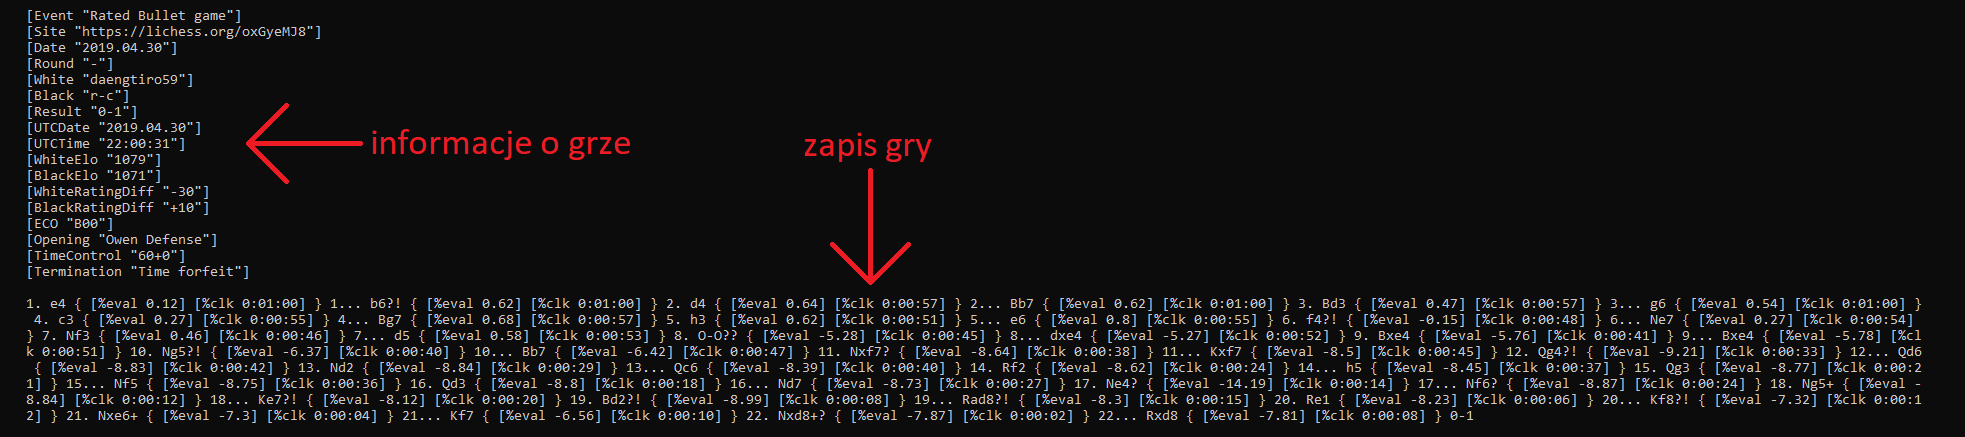
\includegraphics[width=\textwidth]{zapis_gry.png}
	\caption{Przykładowy zapis jednej partii zawierającej ocenę silnika Stockfish}
	\label{rys:zapis_gry} 
\end{figure}
Istotnym problemem związanym z danymi jest dokładność pozostałego czasu jedynie do sekund, co zaburza lekko ich istotę, szczególnie podczas analizy gier w krótszym formacie czasowym (jak np. ,,60+0''), gdzie ułamki sekundy są  znaczące. Dodatkowo ruch, który oznaczony został jako n sekund w rzeczywistości jest ruchem z przedziału obustronnie otwartego (n-1,n+1) sekund. Przy dużej liczbie danych nie ma to jednak większego znaczenia, ponieważ zgodnie z Prawem Wielkich Liczb można takie dane uśrednić do \textit{n} \textbf{cite???}. Jedynym problemem, który może się pojawić jest późniejsze sprawdzenie zgodności danych z rozkładem. 

\subsection{Odfiltrowanie danych}

Pierwszym krokiem potrzebnym do wykonania analizy jest odfiltrowanie danych.
Po rozdzieleniu pliku tekstowego na kolejne gry, pozostawione zostały jedynie te, które zostały wcześniej ocenione przez silnik oraz grane były w formacie ,,300+0'' lub ,,600+0''. Następnie przygotowany wcześniej program zbadał każdy ruch każdej gry i przypisał do niego następujące atrybuty:
\begin{itemize}
	\item game\_ID -- numer gry
	\item score -- ocena ruchu według silnika Stockfish
	\item delta\_time -- czas na wykonanie danego ruchu
	\item WhiteElo -- ranking białych
	\item BlackElo -- ranking czarnych
	\item TimeControl -- czas na wykonanie ruchów każdego z graczy w formacie  ,,sekundy + sekundy dodane za wykonanie ruchu''
	\item color -- gracz, wykonujący dany ruch
	\item move -- numer ruchu w danej partii
	\item result - wynik partii
\end{itemize}

Stworzona baza zawiera 17 524 012 posunięć ze 275 994 gier, co daje średnią 31,75 ruchu na grę (jeden ruch oznacza posunięcie białych i czarnych). Fragment bazy przedstawiony został na rysunku \ref{rys:baza_ruchow}. 
\begin{figure}[H]
	\centering
	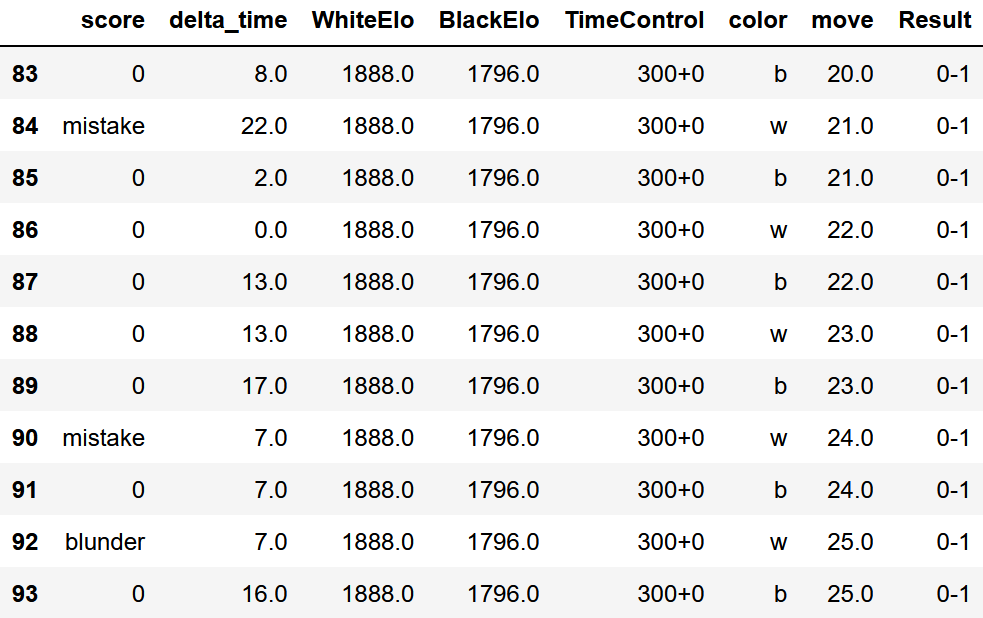
\includegraphics[width=\textwidth]{danee.png}
	\caption{Fragment bazy zawierającej ruchy z gier o formatach czasowych ,,300+0'' i ,,600+0''.}
	\label{rys:baza_ruchow}
\end{figure}




\section{Analiza problemu}

\subsection{Wstępny przegląd danych}



Pierwszym problemem, który zostanie poruszony jest zbadanie statystycznej zależności jakości wykonanego ruchu według oceny silnika Stockfish od czasu potrzebnego na jego wykonanie. W celu uzyskania bardziej precyzyjnych wyników pierwsze 4 ruchy (po 4 posunięcia białych i czarnych) nie będą brane pod uwagę. Są one elementem teorii otwarć szachowych \footnote{ Jedyne otwarcia, które składają się z mniej niż czterech ruchów są wariancjami otwarcia \textit{Fool's Mate}, które prowadzi do zakończenia gry w dwóch lub trzech ruchach, bądź sekwencjami posunięć, które nie mają logicznych podstaw.}, w związku z czym wykonywane są zazwyczaj bardzo szybko i ze znikomą szansą popełnienia błędu, co może powodować zaburzenie danych. Dodatkowo na stronie \textit{Lichess.com} pierwszy ruch obydwu zawodników zawsze zabiera 0 sekund.

Przy analizie z uwzględnieniem rankingu graczy, zastosowane będą podziały kwartylowe. Rozkład rankingu wraz z zaznaczonymi kwartylami pokazany jest na rysunku \ref{rys:rozklad_elo}. Jak widać zbiega on do rozkładu normalnego. Anomalia dla rankingu 1500 związana jest z tym, że jest to ranking przyznawany każdemu graczowi przy jego pierwszej rozgrywce na platformie.
\begin{figure}[H]
	\centering
	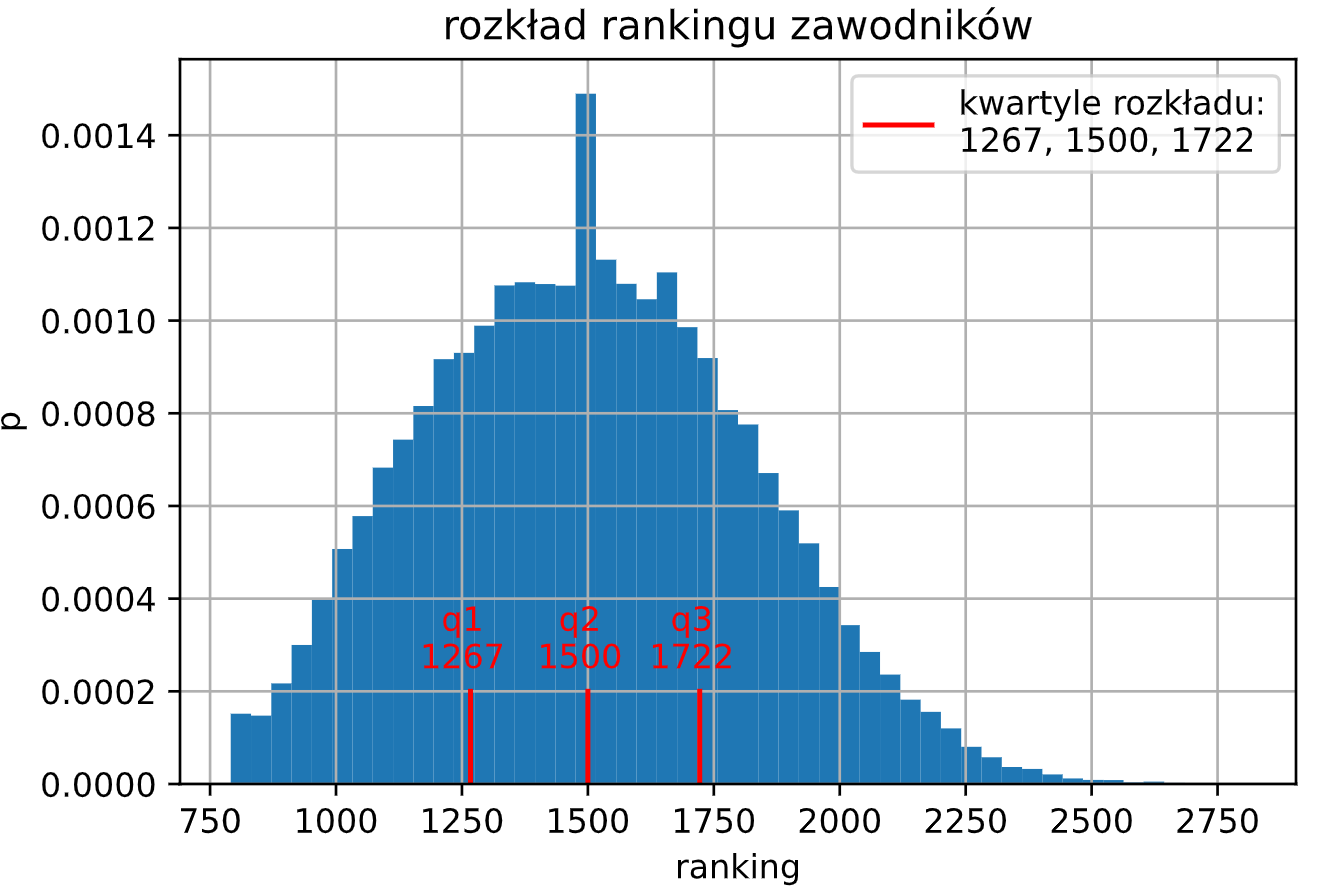
\includegraphics[width=\textwidth]{ranking.png}
	\caption{rozkład rankingu zawodników wraz z zaznaczonymi kwartylami}
	\label{rys:rozklad_elo}
\end{figure}
W późniejszej części pracy pojawią się wykresy i analizy, w których dziedziną będzie numer wykonywanego ruchu. W związku z bardzo małą liczbą danych dla późniejszych ruchów, ich analiza jest zaburzona i niewiarygodna. Dlatego analizowane będą jedynie ruchy z indeksem poniżej 59, jako, że wynik 95\% gier pojawia się maksymalnie w 58 ruchach. Rozkład długości gier z bazy danych, który obrazuje przedstawioną sytuację zamieszczony jest na rysunku \ref{rys:dlugosc_gier}.

\begin{figure}[h]
	\centering
	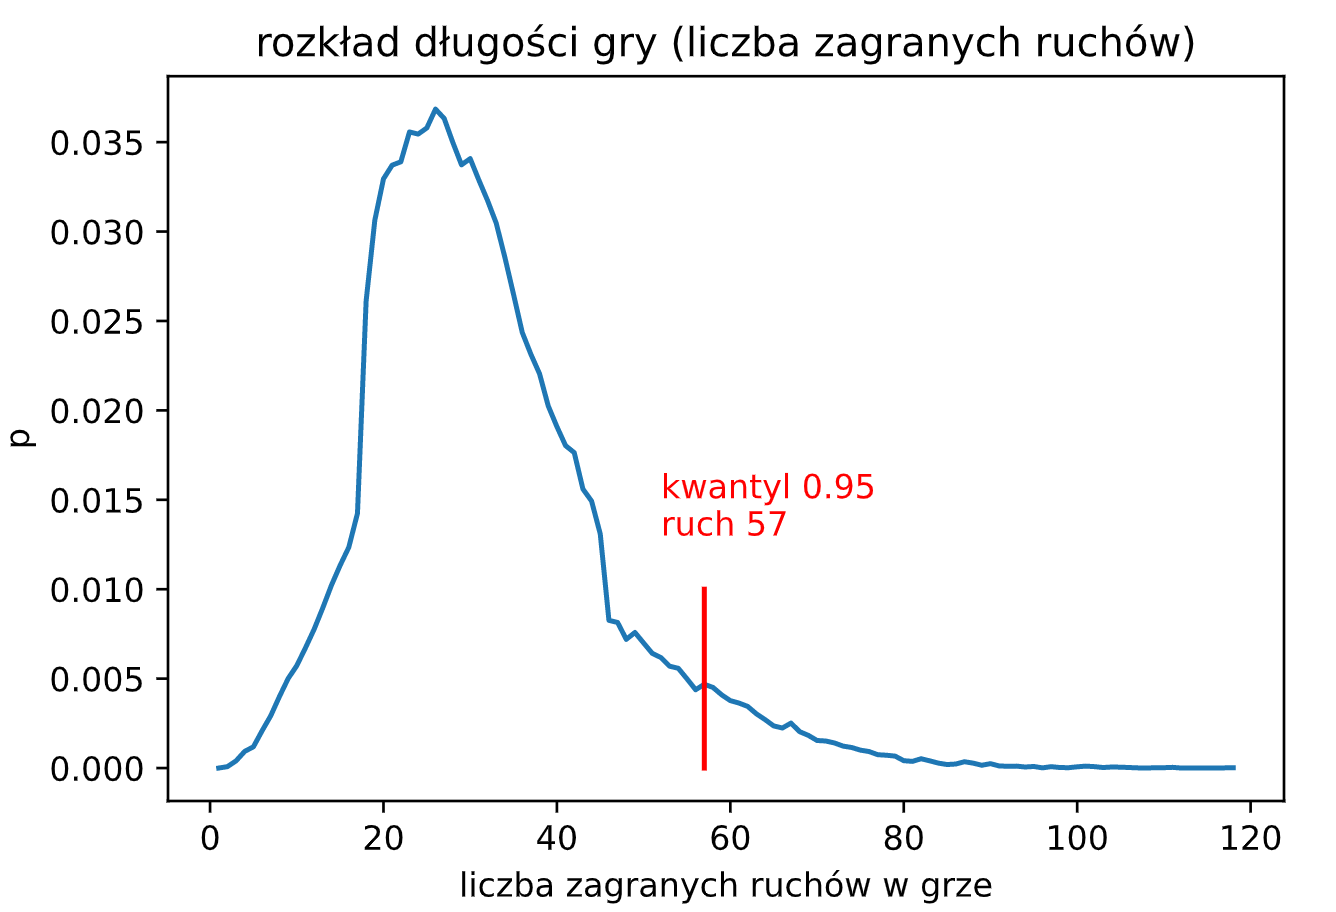
\includegraphics[width=\textwidth]{dlugosc_gry.png}
	\caption{rozkład długości gier wraz z zaznaczonym kwantylem rzędu 0.95,  dla gier z formatu 300+0 oraz 600+0.}
	\label{rys:dlugosc_gier}
\end{figure}


\subsection{Zależność między indeksem ruchu, a poświęconym czasem}


Na początku tej części trzeba ustalić pewne założenia dotyczące zestawu danych. W pojedynczej grze szachowej często występuje sytuacja, w której gracz długo myśli nad konkretnym posunięciem, rozpatrując możliwe następujące po nim sekwencje. W określonych okolicznościach, takich sekwencji jest na tyle mało, że każdy z graczy ma przez kilka kolejnych ruchów tylko jedno nieprzegrywające, łatwe do znalezienia posunięcie. Czas na wykonanie takich ruchów jest więc od siebie w pewien sposób zależny, jednakże sytuacje takie pojawiają się na bardzo nieoczekiwanie i przez mnogość zmiennych są trudne do znalezienia i uwzględnienia. Dlatego w celu ułatwienia analizy, w dalszych rozważaniach następujące po sobie ruchy będą uznawane za niezależne względem siebie.
\begin{figure}[H]
	\centering
	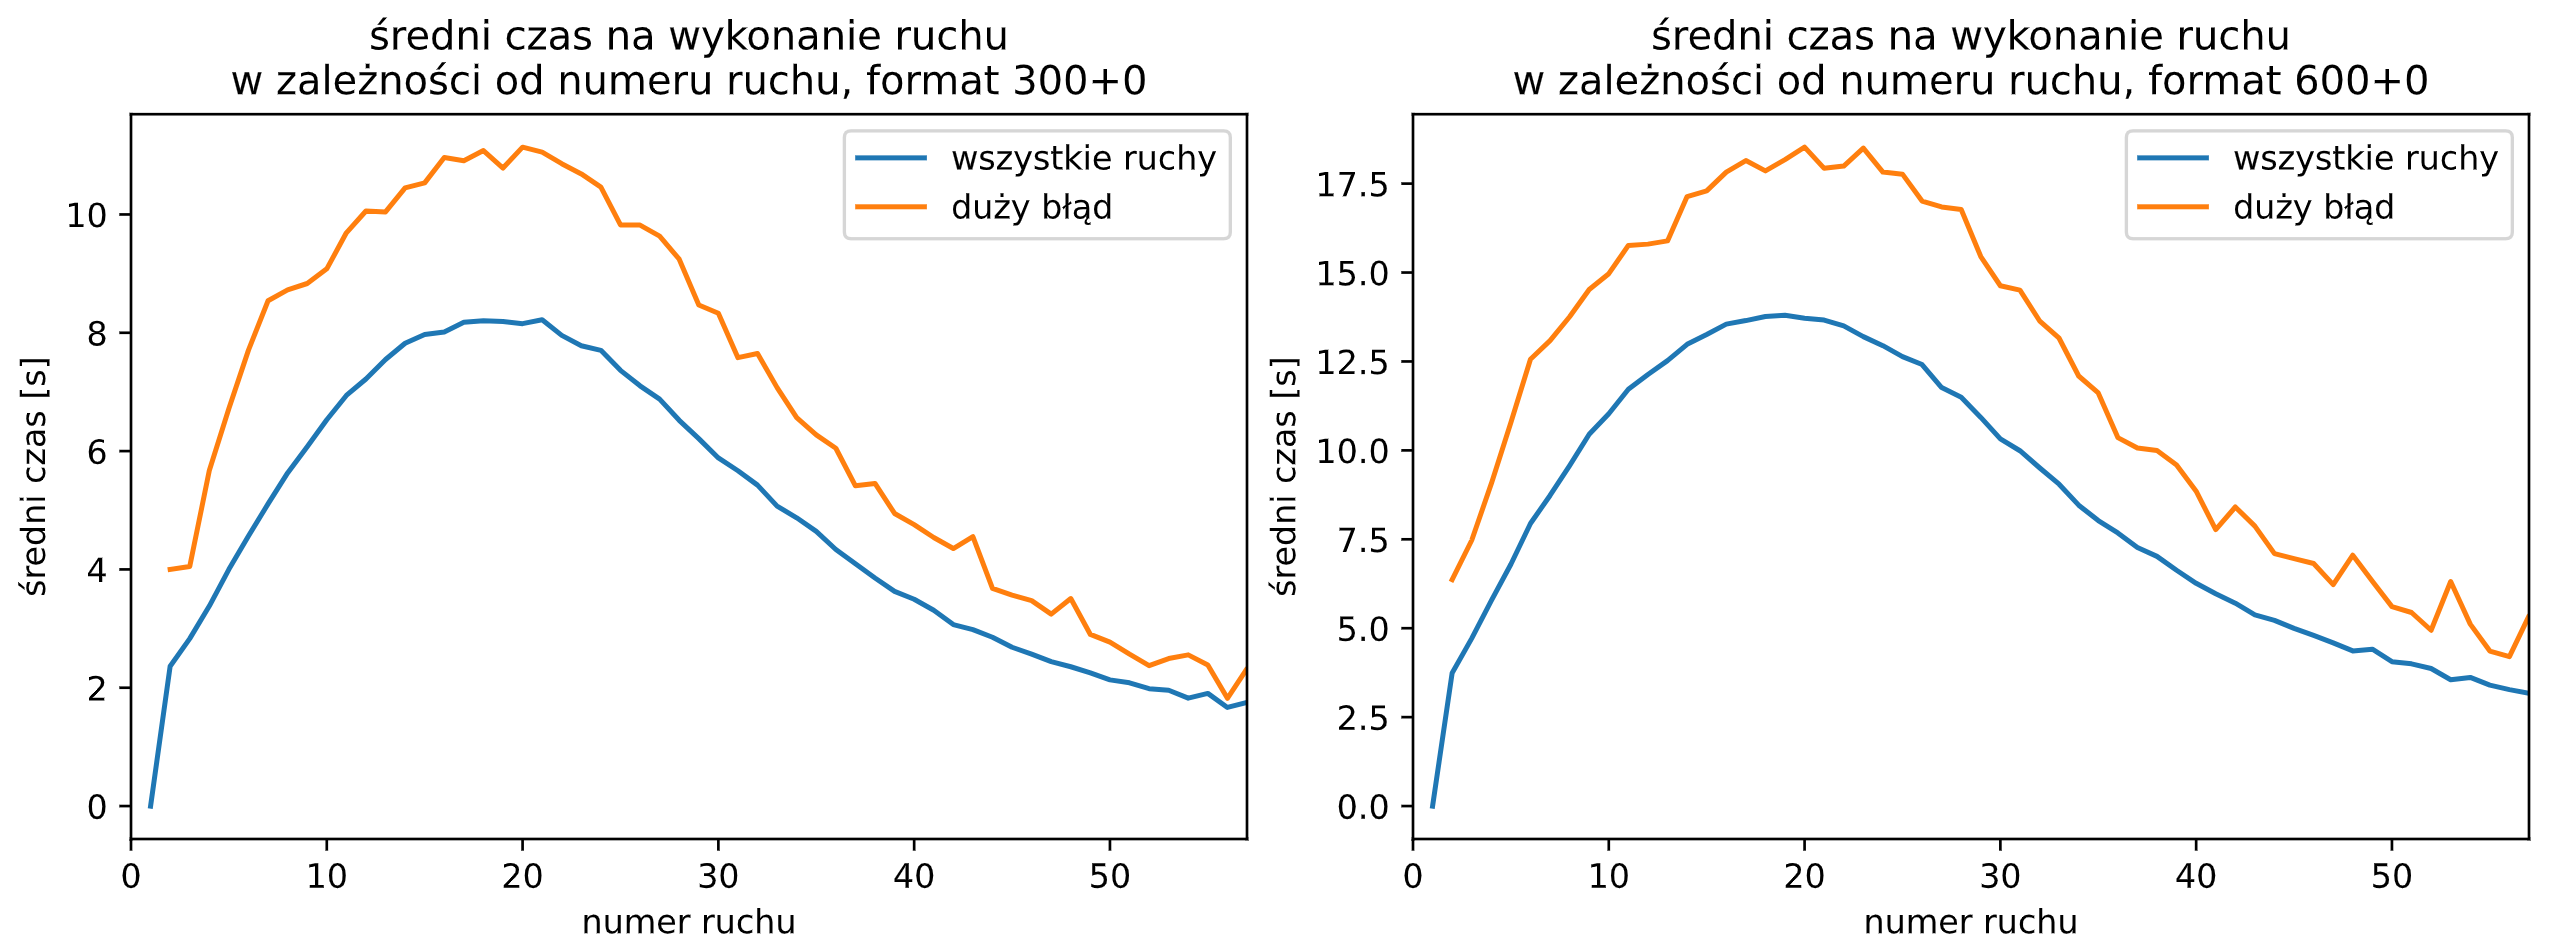
\includegraphics[width=\textwidth]{sr_czas_na_ruch.png}
	\caption{Średni czas na wykonanie ruchu dla analizowanych formatów czasowych wraz z zaznaczonym rozstępem międzykwartylowym. Osobno wszystkie ruchy i ruchy oznaczone przez silnik jako błąd.}
	\label{rys:sr_czas_na_ruch}
\end{figure}

Pierwszym elementem analizy, który pozwoli na określenie wstępnej różnicy między ruchami oznaczonymi jako błąd, a zbiorem wszystkich ruchów jest sprawdzenie zależności między indeksem ruchu, a średnim czasem na jego wykonanie dla obydwu zbiorów. Intuicja wskazuje, że błąd popełniamy poświęcając mniej czasu na ruch. Jak widać na rysunku \ref{rys:sr_czas_na_ruch}, dla każdego analizowanego ruchu, ruch oznaczony jako błędny zajął statystycznie więcej czasu - zarówno dla formatu 300+0 jak i 600+0, co przeczy intuicji. 
Przyczyną tego może być zaliczanie do zbioru wszystkich ruchów posunięć oczywistych, zajmujących niewielką ilość czasu, następujących dla pozycji, w której gracze na każdym poziomie zaawansowania rzadko kiedy popełniają błędy.
Kolejną przyczyną takiego stanu rzeczy może być oczywista zależność skomplikowania pozycji od szansy na popełnienie błędu. W trudnych sytuacjach na szachownicy błędów pojawia się po prostu więcej, a trudnych sytuacji najwięcej jest w środkowej części partii, przez mnogość figur i możliwych legalnych ruchów. Trudno też znaleźć takie pozycje, ponieważ zależą one od przyjętej miary, o czym pisze D. H. Holding w swojej pracy zatytuowanej \textit{,,Evaluation of Chess Positions''} \cite{Holding1979TheEO}.  Dlatego też, co dobrze widoczne jest na wykresie, w środkowej części gry posunięcia zajmują najwięcej czasu.

Po oznaczeniu \textit{D} jako zmienną określającą skomplikowanie pozycji, \textit{T} - zmienną określającą czas na wykonanie ruchu w danej pozycji, \textit{B} - zdarzenie polegające na tym, że posunięcie jest błędne i przy założeniu, że \textit{T} jest silnie dodatnio skorelowane z \textit{D}, według prawdopodobieństwa otrzymujemy %\textbf{SPRAWDZIĆ TO JESZCZE!}:
\begin{equation}
	P(B|D>d_0) > P(B|D\leq d_0) \rightarrow P(B|T>t_0) > P(B|T\leq t_0)
\end{equation}
gdzie $d_0$ i $t_0$ określają punkty, od których według wybranej miary można określić, że pozycja jest skomplikowana ($D>d_0$) i czas na wykonanie posunięcia jest długi ($T>t_0$).


Może to tłumaczyć wyższą średnią czasu na wykonanie błędnego posunięcia w porównaniu do zbioru wszystkich posunięć.
\begin{figure}[h]
	\centering
	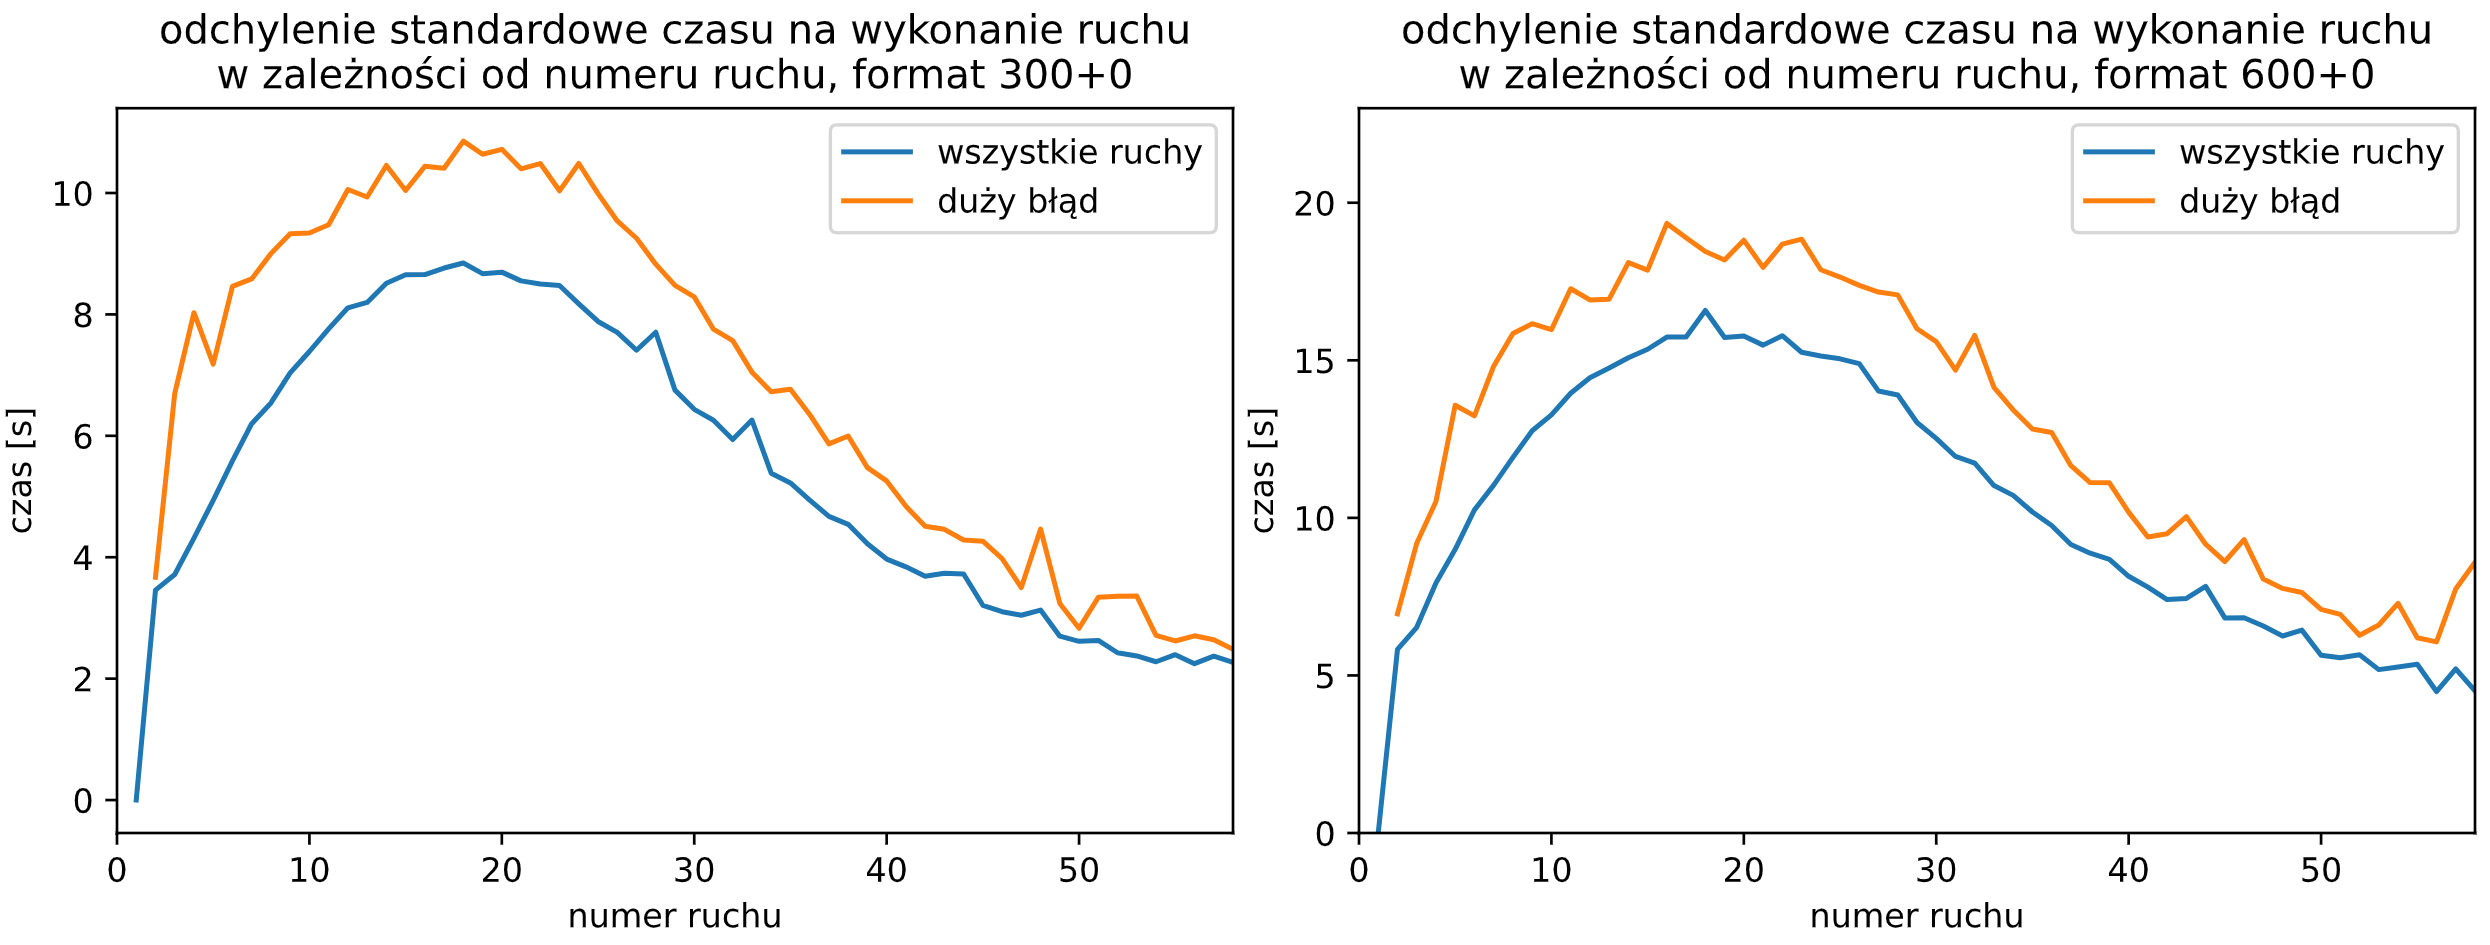
\includegraphics[width=\textwidth]{std_czas_na_ruch.png}
	\caption{Odchylenie standardowe czasu na wykonanie ruchu dla analizowanych formatów czasowych. Osobno wszystkie ruchy i ruchy oznaczone przez silnik jako błąd.}
	\label{rys:std_czas_na_ruch}
\end{figure}

Badając w dalszym ciągu wykresy na rysunku \ref{rys:sr_czas_na_ruch} można zauważyć, że dla obydwu zbiorów posunięć początkowo niska średnia osiąga swój szczyt w okolicach dwudziestego ruchu, by później stopniowo się zmniejszać. Ma to związek z tym, że początkowe posunięcia są elementem teorii szachowej. Spora część graczy nauczyła się kilku, kilkunastu, bądź w przypadku gry na najwyższym poziomie - nawet ponad dwudziestu pierwszych ruchów niektórych otwarć. W związku z tym początkowe ruchy grane są relatywnie szybko. Końcowe posunięcia natomiast nie mogą zająć wiele czasu, ponieważ jest go zazwyczaj zbyt mało na zegarze, by gracz mógł sobie na to pozwolić. Dlatego też od pewnego momentu, wraz ze wzrostem indeksu średni czas poświęcony na ruch zbiega do zera. Zaznaczone na rysunku rozstępy międzykwartylowe dla każdego ruchu wskazują na znacznie większą wariancję czasu na wykonanie błędnego ruchu porównując do zbioru wszystkich ruchów. Potwierdza to rysunek \ref{rys:std_czas_na_ruch} pokazujący odchylenie standardowe dla kolejnych ruchów. 
\begin{figure}[h]
	\centering
	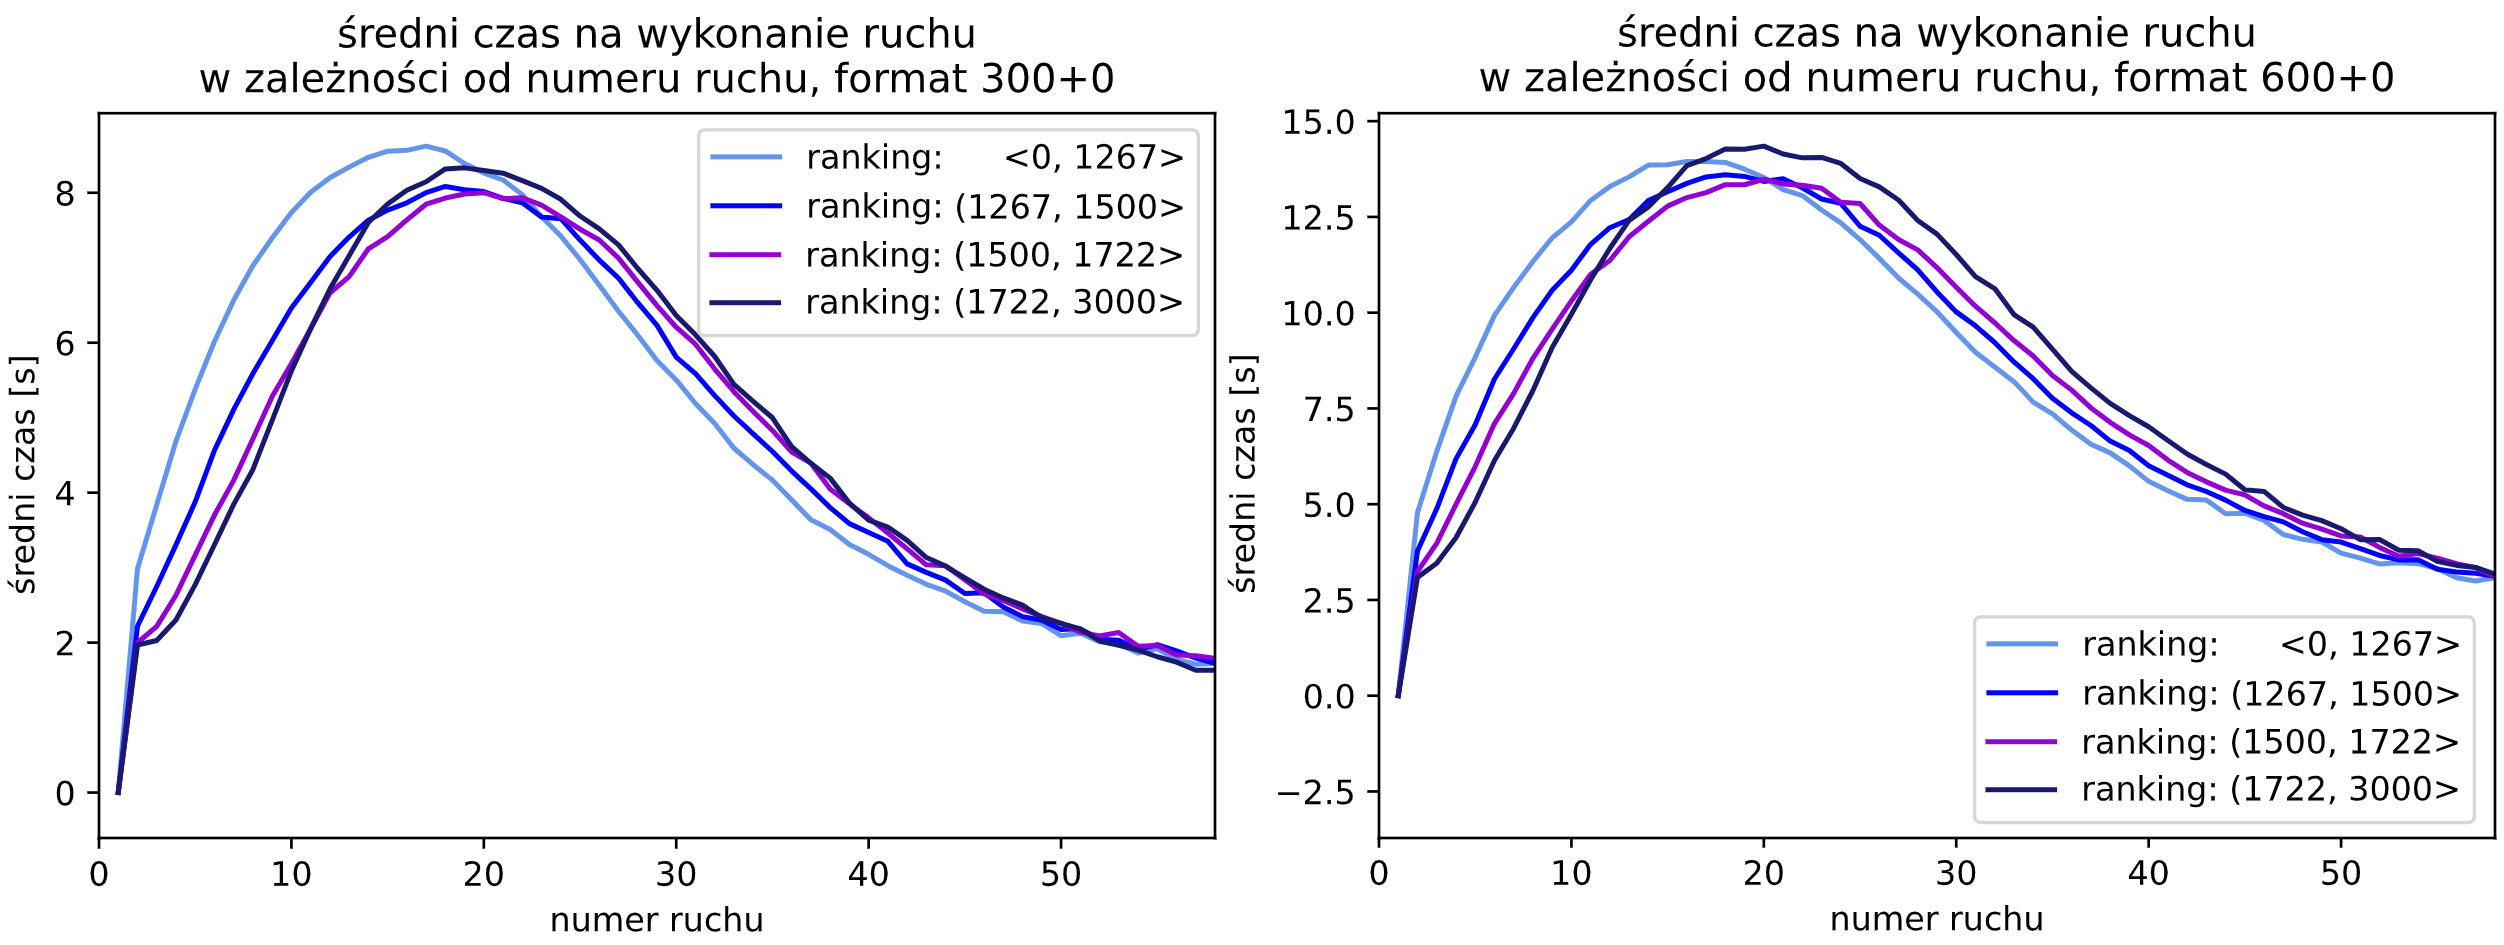
\includegraphics[width=\textwidth]{sr_czas_na_ruch_ELO_1.png}
	\caption{Średni czas na wykonanie ruchu dla graczy z różnych przedziałów rankingowych. Wszystkie posunięcia.}
	\label{rys:sr_czas_na_ruch_ELO_1}
\end{figure}

Rysunki \ref{rys:sr_czas_na_ruch_ELO_1} i \ref{rys:sr_czas_na_ruch_ELO_2} wprowadzają do rozważań różnicę między średnim czasem na wykonanie ruchu dla graczy z poszczególnych przedziałów rankingowych. Można zauważyć, że zarówno w przypadku zbioru wszystkich ruchów (rysunek \ref{rys:sr_czas_na_ruch_ELO_1}) jak i pozdbioru ruchów błędnych (rysunek \ref{rys:sr_czas_na_ruch_ELO_2}), słabsi gracze mają tendencję do dłuższych rozważań nad początkowymi ruchami. Wraz ze wzrostem rankingu wydłuża się średni czas na wykonanie ruchu dla ruchów z indeksem od 20 do 30 - czyli tych, gdzie średnia jest najwyższa. Przy końcowych posunięciach, posunięcia zajmują podobną ilość czasu dla wszystkich rankingów. Warto zwrócić uwagę, że odsetek 25\% najniżej notowanych graczy przez zbyt długie początkowe ruchy zmuszona jest ruszać się szybciej w późniejszych posunięciach. Szczególnie widoczne jest to na pierwszym wykresie rysunku \ref{rys:sr_czas_na_ruch_ELO_2}. 

\begin{figure}[h]
	\centering
	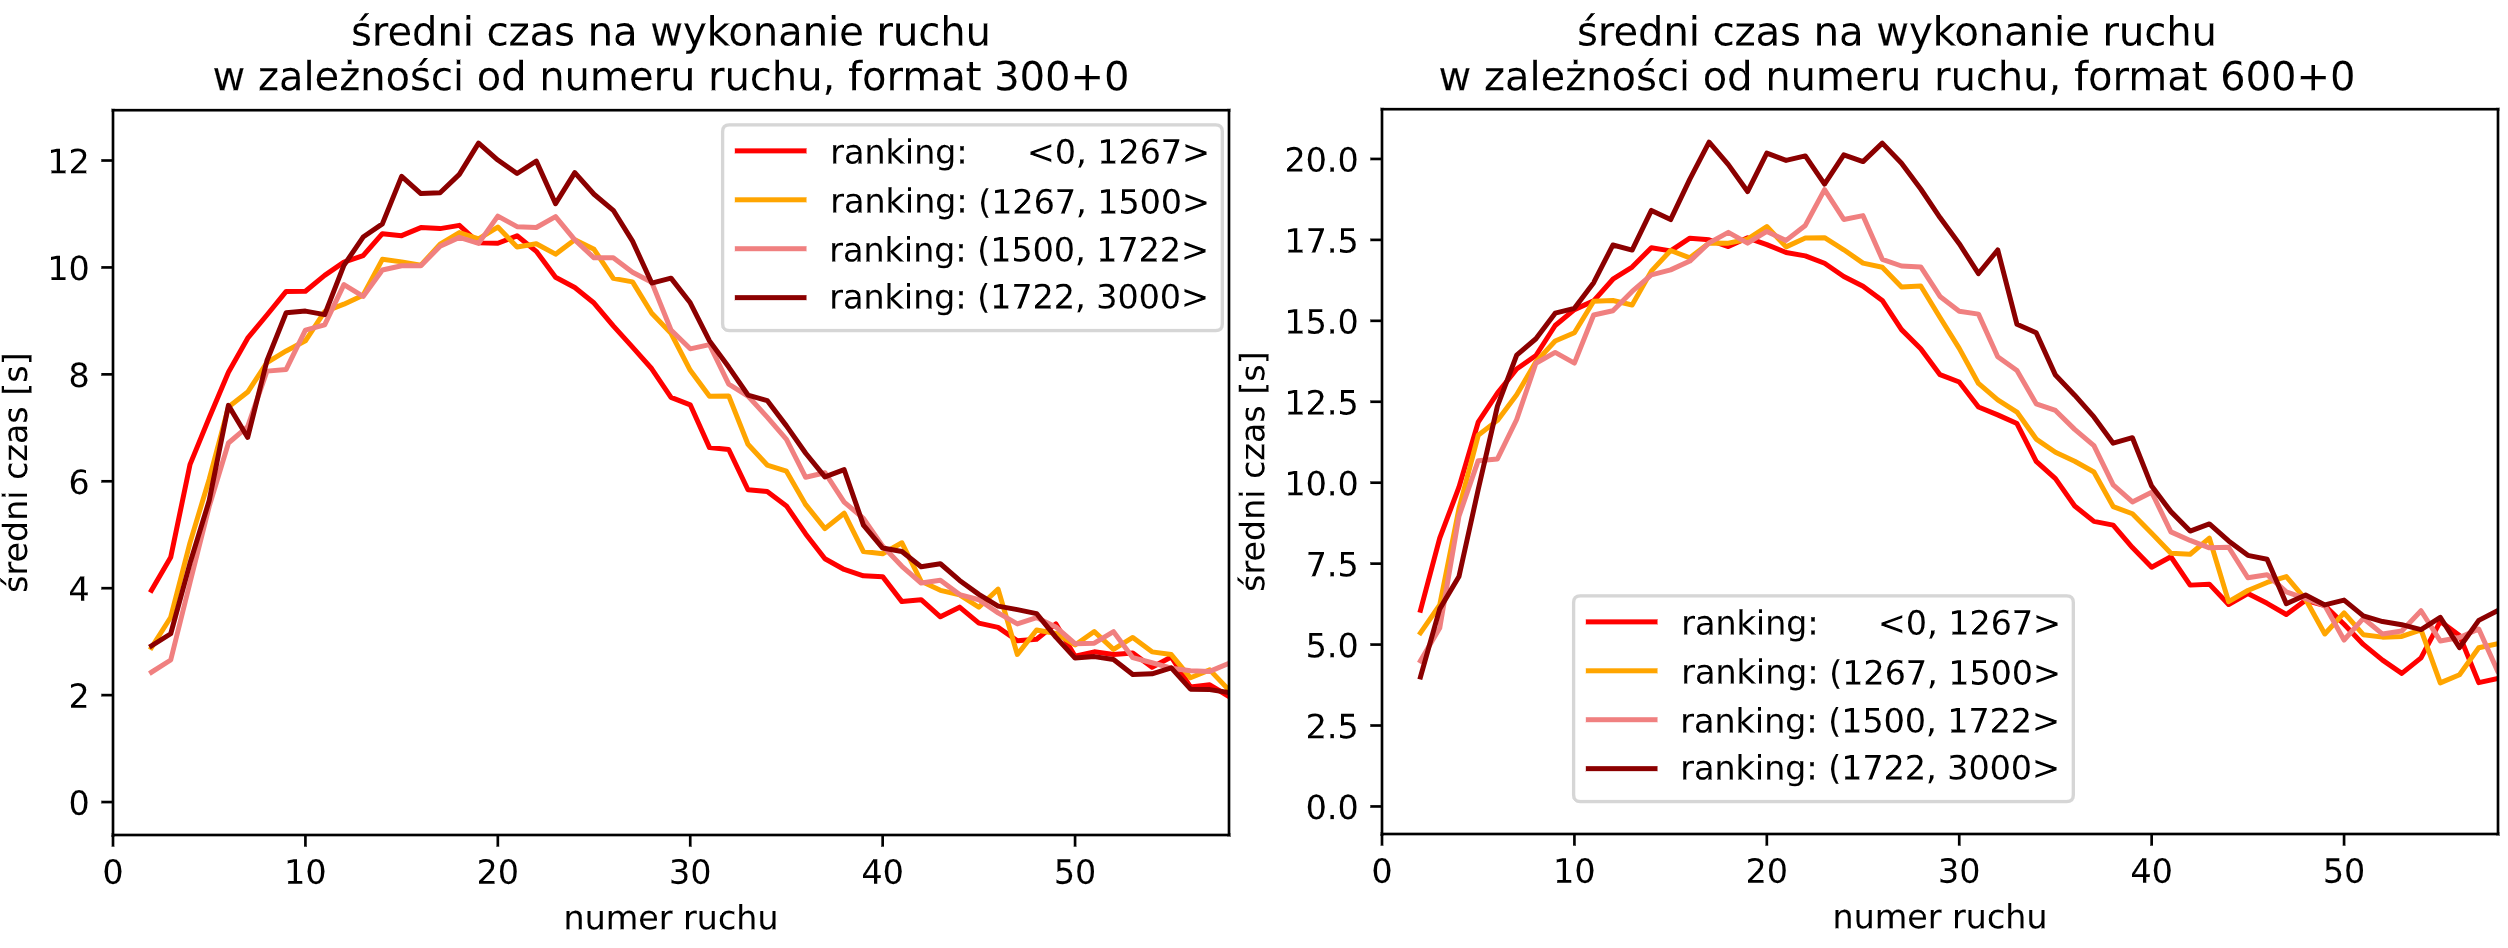
\includegraphics[width=\textwidth]{sr_czas_na_ruch_ELO_2.png}
	\caption{Średni czas na wykonanie ruchu dla dla graczy z różnych przedziałów rankingowych. Posunięcia oznaczone przez silnik jako błąd.}
	\label{rys:sr_czas_na_ruch_ELO_2}
\end{figure}
Niezależnie od rankingu, średnia poświęconego czasu dla posunięć oznaczonych przez silnik jako błąd jest w każdym momencie wyższa niż dla zbioru wszystkich ruchów. 
Warto również zauważyć, że wykresy dla obydwu formatów czasowych wyglądają podobnie. 
\begin{figure}[h]
	\centering
	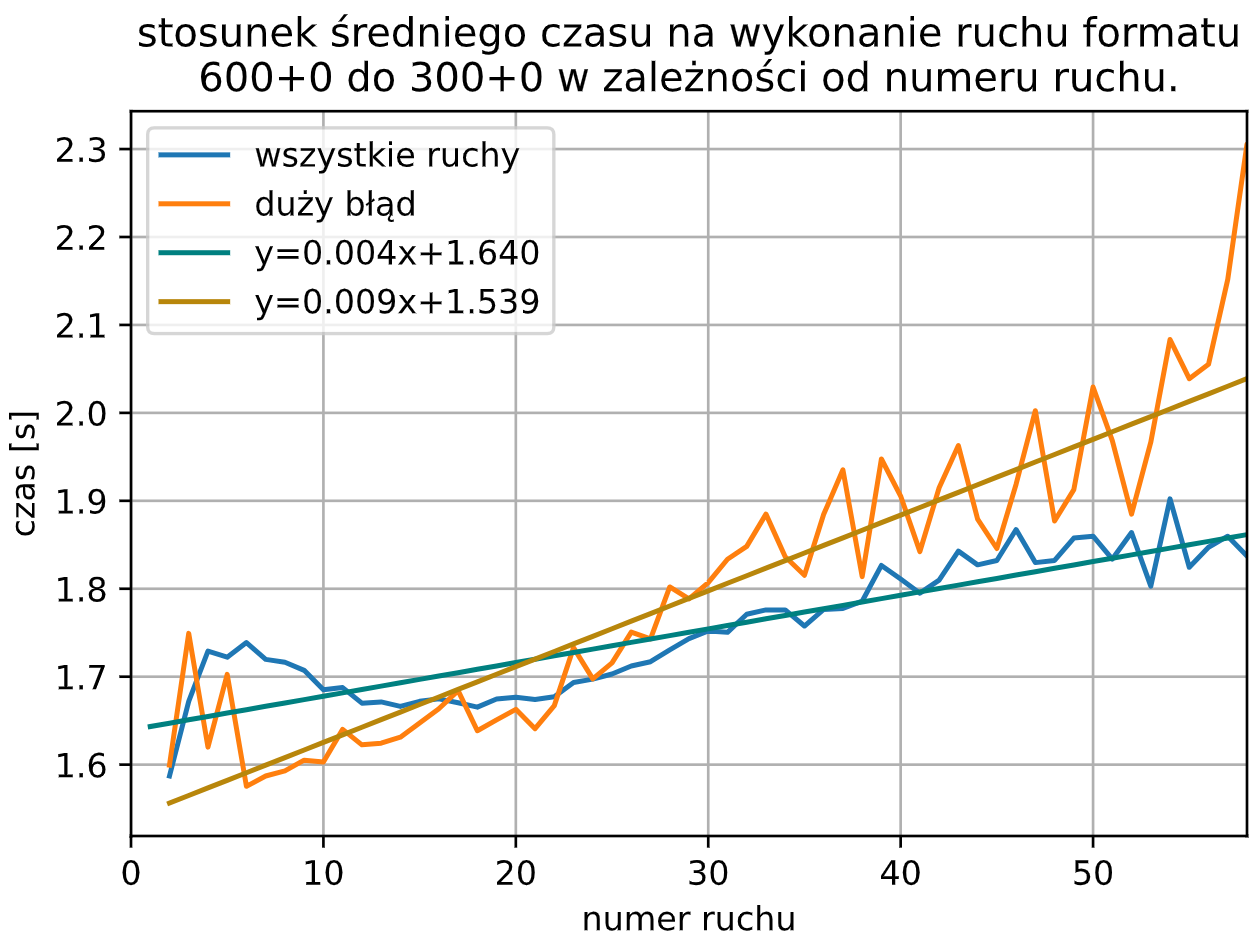
\includegraphics[width=\textwidth]{stosunek_sr_czas.png}
	\caption{Stosunek średniego czasu na wykonanie ruchu w formacie 600+0 do czasu w formacie 300+0. Zaznaczone proste regresji obrazujące trend.}
	\label{rys:stosunek_sr_czas}
\end{figure}
By móc przeanalizować zależność między rozgrywanym formatem, a wzrostem średniego czasu poświęconego na ruch, powstał wykres umieszczony na rysunku \ref{rys:stosunek_sr_czas}. Dopasowane metodą najmniejszych kwadratów opisanej w rozdziale \ref{teoria} proste regresji obrazują różnice w zachowanych trendach. Czas w formacie 600+0 jest dokładnie 2 razy dłuższy niż w formacie 300+0, jednak średni czas na wykonanie ruchu jest w pierwszym przypadku około 1,7 raza wyższy. Wartość stosunku jednak nie jest stała i wzrasta wraz z indeksem ruchu. Dla zbioru wszystkich posunięć dopasowana prosta regresji wskazuje na stosunek około 1,65 dla tych początkowych, do 1,85 przy końcowych. Znacznie większa rozpiętość w stosunku widoczna jest dla posunięć oznaczonych jako błąd. Stosunek wynosi około 1,55 dla początkowych wartości i powyżej 2 dla ruchów z indeksem powyżej 55. Warto zauważyć, że dla obu zbiorów w formacie 600+0 gracze nie są zmuszeni do podejmowania decyzji pod dużą presją czasu. Szczególnie różnicę tę da się zauważyć dla ruchów błędnych, nad którymi gracz musi się statystycznie dłużej zastanowić (rysunek \ref{rys:sr_czas_na_ruch} na stronie \pageref{rys:sr_czas_na_ruch}). Gracz posiadając 2 razy więcej czasu w tym formacie i myśląc nad każdym ruchem średnio od 1.55 do 1.95 raza dłużej,  ma w każdym momencie gry do dyspozycji statystycznie większy ułamek początkowego czasu niż w przypadku gry w formacie 300+0. Zestawienie pozostałego czasu pokazane jest na pierwszym wykresie na rysunku rysunku \ref{rys:pozostaly_czas}. Widać dość sporą różnicę w średnim pozostałym czasie narastającą podczas przebiegu gry. Drugi wykres zamieszczony na rysunku ukazuje różnicę w prawdopodobieństwie popełnienia błędu w konkretnym ruchu dla obu formatów. Warto zauważyć, że mimo znacznie większego czasu do dyspozycji w przypadku formatu ,,600+0'', do 20 ruchu szansa na błąd jest niemalże identyczna jak w przypadku formatu ,,300+0'' -- Krzywe odbiegają od siebie nieznacznie. W okolicach od 20 do 40 ruchu, szansa na popełnienie błędu w formacie ,,300+0'' jest około 5-10\% większa. Dobrze jest w tym miejscu dodać, że jest to przedział, w którym błędów występuje najwięcej.


\begin{figure}[h]
	\centering
	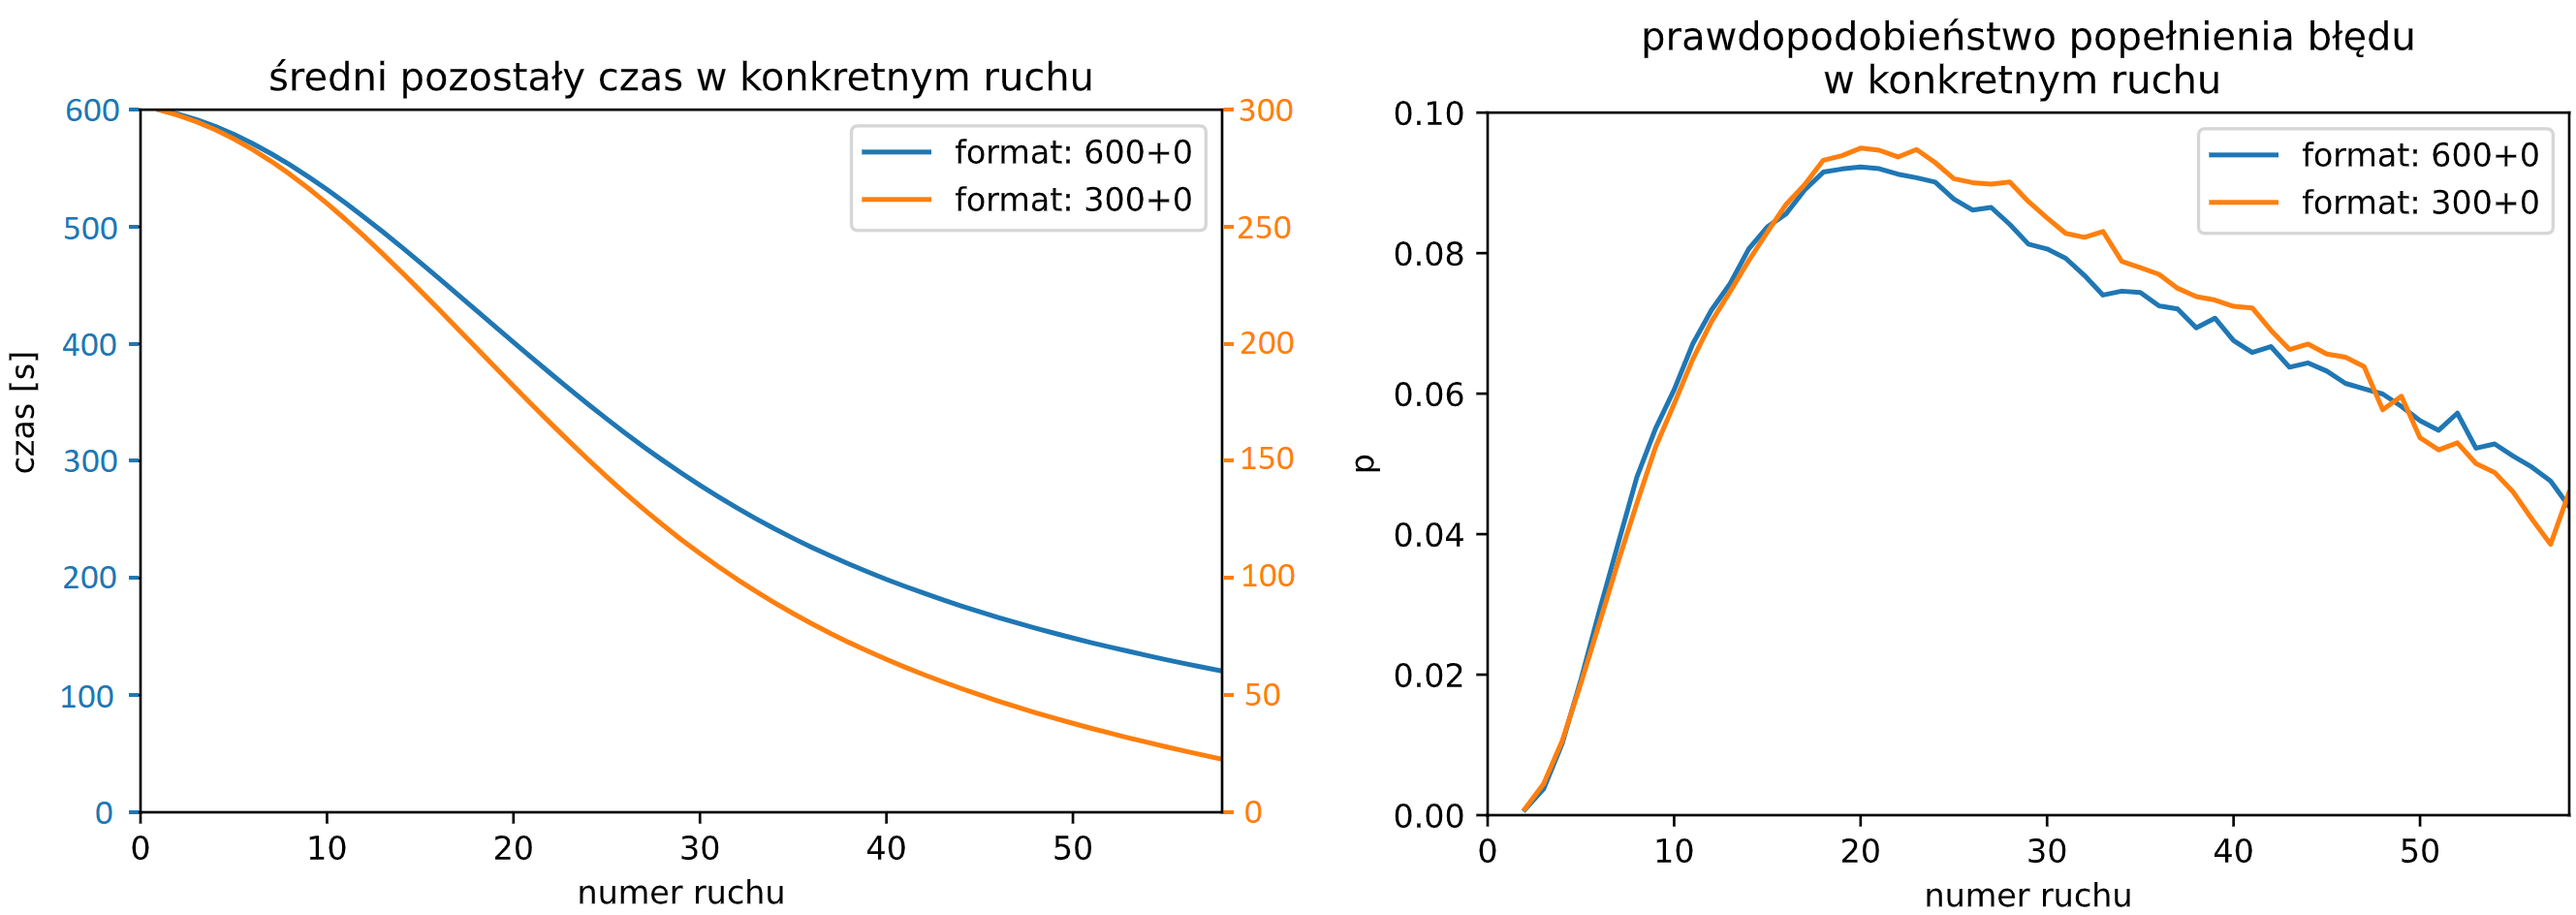
\includegraphics[width=\textwidth]{pozostaly_czas.png}
	\caption{
		Pierwszy wykres -- zestawienie średniego pozostałego czasu w formatach 600+0 oraz 300+0. W celu lepszego porównania zastosowane osobne osie dla każdego formatu. Drugi wykres -- empiryczne prawdopodobieństwo popełnienia błędu w konkretnym ruchu.}
	\label{rys:pozostaly_czas}
\end{figure}
\begin{figure}[h]
	\centering
	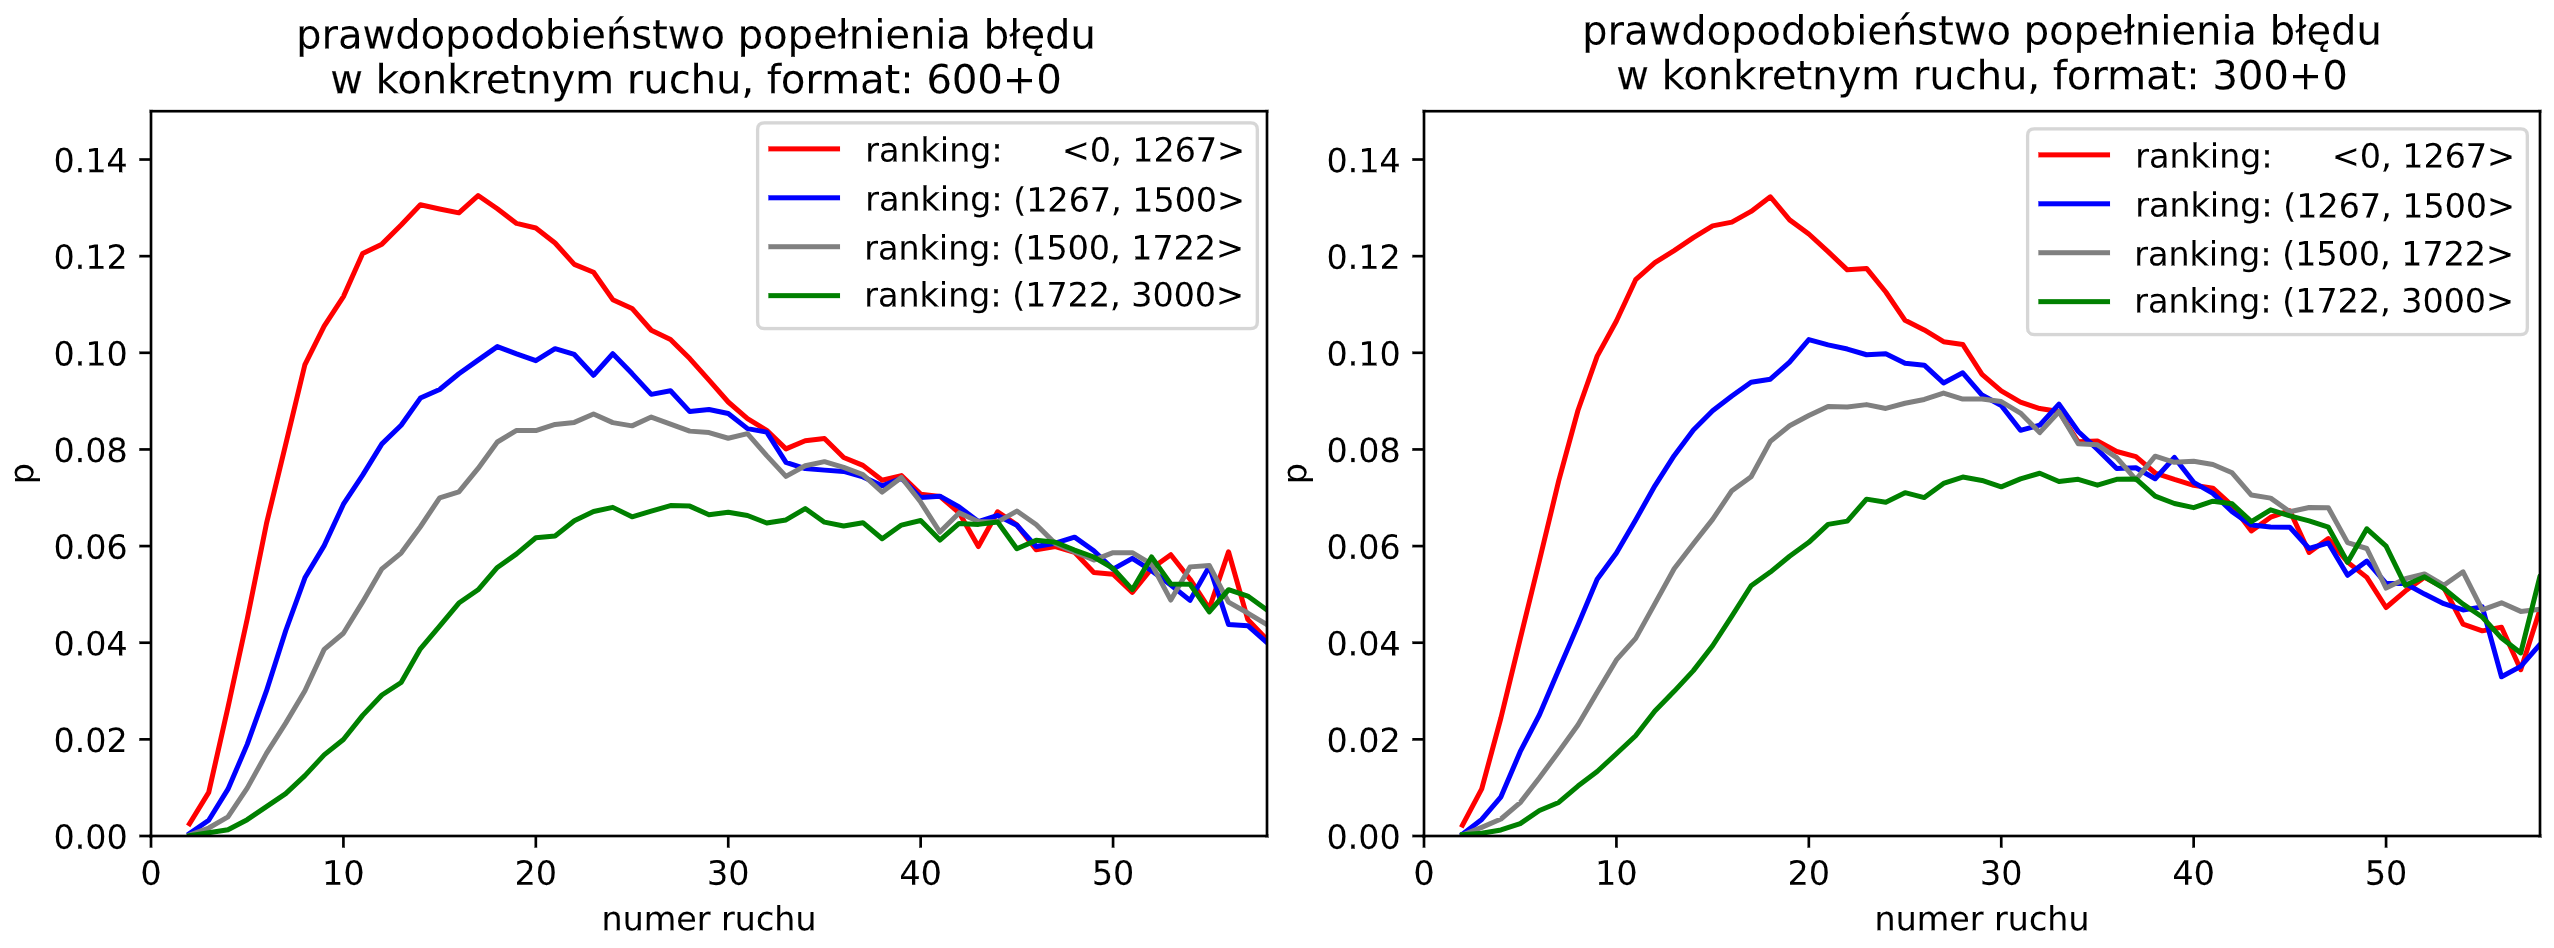
\includegraphics[width=\textwidth]{prawd_blad_ELO.png}
	\caption{Prawdopodobieństwo popełnienia błędu w konkretnym ruchu dla różnych przedziałów rankingowych.}
	\label{rys:prawd_blad_ELO}
\end{figure}
Różnica w prawdopodobieństwie popełnienia błędu pomiędzy poszczególnymi formatami nie jest tak duża jak ta pomiędzy rankingiem graczy. Na rysunku \ref{rys:prawd_blad_ELO} można zauważyć, że dla zarówno dla formatu ,,600+0'' jak i ,,300+0'' słabsi gracze mają tendencję do popełniania większej liczby błędów w początkowej fazie gry, niż ich wyżej notowani koledzy. Statystycznie, będąc w grupie 25\% najniżej notowanych graczy ma się około 6 razy większe prawdopodobieństwo na popełnienie błędu w 10 posunięciu, niż osoba z grupy 25\% najwyżej notowanych graczy. Format gry ma na to niewielki wpływ. Można wysunąć wniosek, że w przypadku gry pomiędzy dwoma takimi zawodnikami, dwukrotnie zwiększenie czasu niżej notowanego gracza z 5 do 10 minut będzie miało minimalny wpływ na finalny wynik gry (przy założeniu, że liczba błędów jest mocno skorelowana z wynikiem gry). krzywe zaczynają do siebie zbiegać od okolic 20 ruchu, by stać się praktycznie nierozróżnialne w okolicach 40 ruchu.

Wykres zależności prawdopodobieństwa od ruchu jest tym bardziej ,,spłaszczony'' im wyższa jest notacja elo zawodników. Brak szybkiego wzrostu dla początkowych posunięć sprawia, że statystyczne prawdopodobieństwo popełnienia błędu w pierwszych 10 ruchach niesamowicie różni się dla poszczególnych grup rankingowych.  Po oznaczeniu przez $X_i$ zmienną losową określającą popełnienie błędu w \textit{i}-tym posunięciu:
\begin{equation*}
X_i =
\begin{cases}
	1, & \text{gdy w $i$-tym ruchu został popełniony błąd}\\
	0, & \text{gdy w $i$-tym ruchu nie został popełniony błąd}
\end{cases}       
\end{equation*}
oraz założeniu, że $X_i$ oraz $X_j$ są niezależne dla $i \neq j$ (drugie przejście w równaniu poniżej \cite[str. 43]{prawdopodobienstwo_wstep}) możemy zbadać empiryczne prawdopodobieństwo popełnienia przynajmniej jednego błędu w \textit{n} pierwszych ruchach.

\begin{multline}
	\begin{split}
	& P(X_1 = 1 \vee X_2 = 1 \vee \dots \vee X_n = 1)  = 1 - P(X_1 = 0, X_2 = 0,\dots, X_n = 0) = \\
	& = P(X_1 = 0)P(X_2 = 0)\dots P(X_n = 0) = \prod_{i=1}^{n}P(X_i=0)
	\end{split}
\end{multline}
Przy czym $P(X_i=0)$ można wyznaczyć empirycznie na podstawie danych.\\

 Tabela \ref{tab:blad_w_n_ruchach} przedstawia różnicę w szansie na popełnienie przynajmniej jednego błędu w pierwszych 10, 20 i 30 ruchach dla graczy z określonych przedziałów rankingowych i gier w określonym formacie. Przykładowo, dla osoby z grupy 25\% najniżej notowanych graczy grającej w formacie ,,600+0'', szansa na popełnienie błędu w 10 pierwszych ruchach wynosi aż 43,46\%, natomiast dla grupy 25\% najlepszych graczy jest to jedynie 6,76\%. Różnica ta zmniejsza się znacząco, gdy weźmie się pod uwagę większą liczbę pierwszych ruchów. Dla 20, jest to kolejno 85,50\% i 40,78\%, a dla 30 -- 95,32\% i 70,27\%. Wartości te wyglądają podobnie dla formatu 300+0.
\begin{table}[H]
	\caption{Szansa na popełnienie błędu w pierwszych \textit{n} ruchach dla gracza z określonego przedziału rankingowego z rozdzieleniem na formaty ,,600+0'' i ,,300+0''}
	\centering
	\begin{tabular}{|l|r|r|r|r|r|r|l}
		\cline{1-7}
		\textbf{\begin{tabular}[c]{@{}l@{}}\textit{n} pierwszych \\ ruchów\end{tabular}} & \multicolumn{2}{l|}{\textbf{n = 10}}                                      & \multicolumn{2}{l|}{\textbf{n = 20}}                                      & \multicolumn{2}{l|}{\textbf{n = 30}}                                      & \textbf{} \\ \cline{1-7}
		\textbf{centyl\hphantom{ } \textbackslash \hphantom{ } format}                                   & \multicolumn{1}{l|}{\textbf{600+0}} & \multicolumn{1}{l|}{\textbf{300+0}} & \multicolumn{1}{l|}{\textbf{600+0}} & \multicolumn{1}{l|}{\textbf{300+0}} & \multicolumn{1}{l|}{\textbf{600+0}} & \multicolumn{1}{l|}{\textbf{300+0}} &           \\ \cline{1-7}
		\textbf{0-25\%}                                                         & 43,36\%                             & 40,72\%                             & 85,50\%                             & 84,33\%                             & 95,32\%                             & 94,96\%                             &           \\ \cline{1-7}
		\textbf{25\%-50\%}                                                      & 25,52\%                             & 22,09\%                             & 71,56\%                             & 68,63\%                             & 89,38\%                             & 88,66\%                             &           \\ \cline{1-7}
		\textbf{50\%-75\%}                                                      & 15,58\%                             & 12,42\%                             & 58,86\%                             & 56,27\%                             & 83,08\%                             & 82,93\%                             &           \\ \cline{1-7}
		\textbf{75\%-100\%}                                                     & 6,76\%                              & 5,63\%                              & 40,78\%                             & 38,66\%                             & 70,27\%                             & 70,40\%                             &           \\ \cline{1-7}
		\textbf{0\%-100\%}                                                     & 23,79\%                              & 22,81\%                              & 67,95\%                             & 67,58\%                             & 87,11\%                             & 87,50\%                             &           \\ \cline{1-7}
	\end{tabular}
	\label{tab:blad_w_n_ruchach} 
\end{table}
W pierwszej części tabeli, dla 10 pierwszych ruchów, co ciekawe, prawdopodobieństwo popełnienia błędu w dłuższym formacie czasowym jest znacznie wyższe niż w krótszym, niezależnie od rankingu zawodnika. Dla większej liczby pierwszych ruchów ta różnica się zmniejsza, jednak cały czas dłuższy format oznacza statystycznie większą szansę na choć 1 popełniony błąd, co wydaje się być sprzeczne z intuicją, ponieważ gracze mają 2 razy więcej czasu na wszystkie posunięcia.

\subsection{zależność między czasem poświęconym na ruch, a jego oceną}


Kolejnym problemem, który zostanie zbadany jest zależność pomiędzy czasem poświęconym na ruch, a jego oceną. Tak jak i we wcześniejszych częściach wartość oceny silnika rozróżniana będzie jedynie na ruchy oznaczone jako błąd i te bez takiego oznaczenia.
\begin{figure}[H]
	\centering
	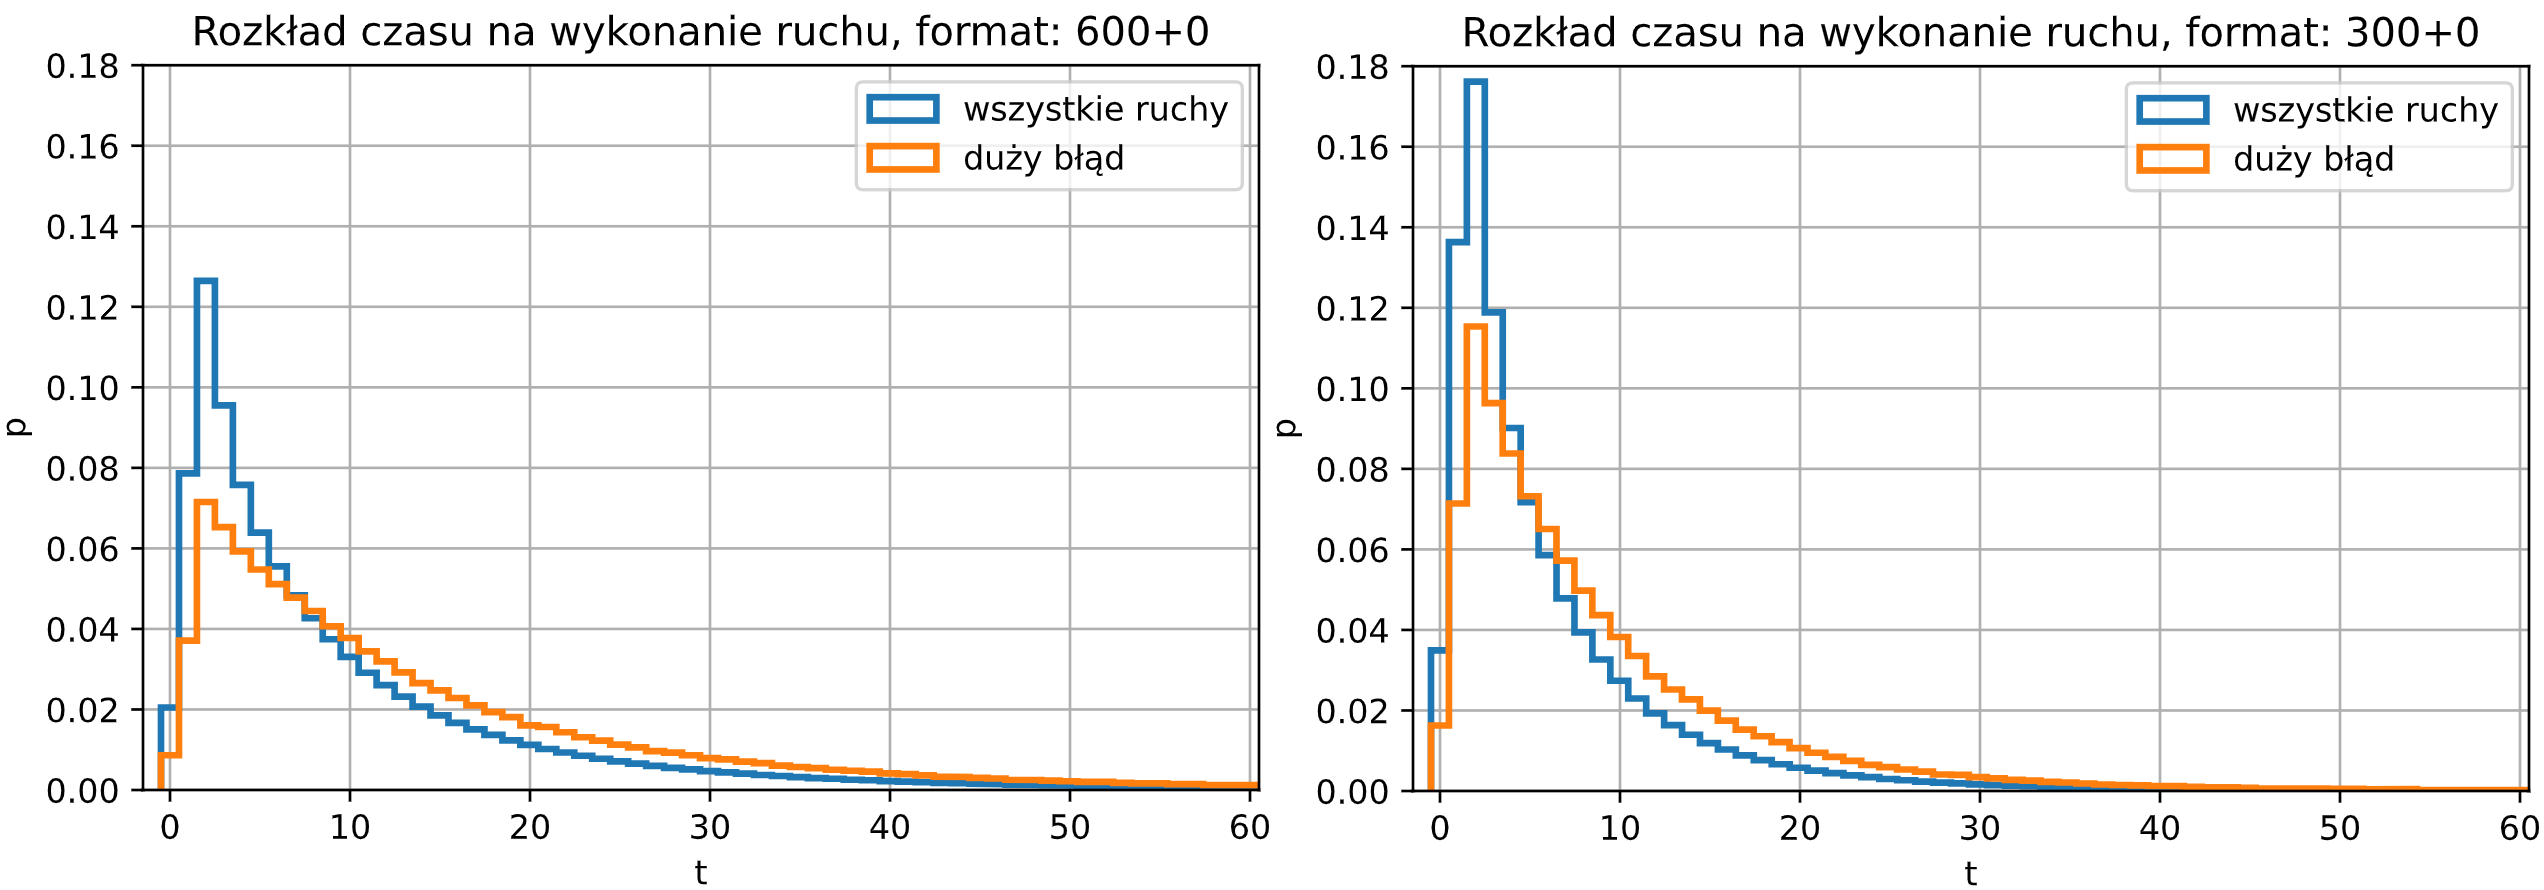
\includegraphics[width=\textwidth]{rozklad_czasu.png}
	\caption{Rozkład czasu poświęconego na wykonanie posunięcia dla formatów ,,600+0'' i ,,300+0''. Osobno wszystkie posunięcia i posunięcia błędne}
	\label{rys:rozklad_czasu}
\end{figure}

Pierwszym spojrzeniem na wymienioną wyżej zależność będzie przeanalizowanie rozkładu czasu na wykonanie ruchu osobno dla zbioru wszystkich ruchów i dla tych błędnych. Jak można zauważyć na rysunku \ref{rys:rozklad_czasu}, w każdym rozważanym formacie czasowym różnica w rozkładzie dla zbioru wszystkich ruchów i zbioru ruchów błędnych jest zauważalna. Oba zbiory mają zachowane podobne tendencje -- najwięcej posunięć zagrywana jest w ciągu od jednej do pięciu sekund. W każdym ze zbiorów wraz ze wzrostem czasu na wykonanie posunięcia, empiryczna gęstość rozkładu się zmniejsza. Ruchów błędnych jest widocznie mniej w porównaniu do zbioru wszystkich ruchów w przedziale od 0 do ok. 8 sekund. Natomiast w przedziale od ok. 8 do 30 sekund, posunięcia błędne są spotykane częściej.
Po przyjrzeniu się danym da się zauważyć, że mogą one pochodzić z rozkładu logarytmicznie-normalnego, co można uwarunkować tym, że w zdecydowanej większości pozycji zawodnik potrzebuje krótkiej chwili na odpowiedź na posunięcie przeciwnika, ponieważ samo zarejestrowanie zmian na planszy i fizyczne wykonanie posunięcia (przesunięcie figury na konkretne pole za pomocą myszki dla komputerów lub przeciągnięcie palcem dla smartfonów) zajmuje pewien czas, wykluczając sytuacje, w których zawodnik dokonuje tzw. ,,premove'', czyli podejmuje decyzję o wykonaniu konkretnego posunięcia zajmującego 0 sekund jeszcze przed zagraniem przeciwnika. Dla formatów ,,300+0'' i ,,600+0'' jest to jednak rzadkością - szczególnie podczas środkowej części gry.

\begin{figure}[h]
	\centering
	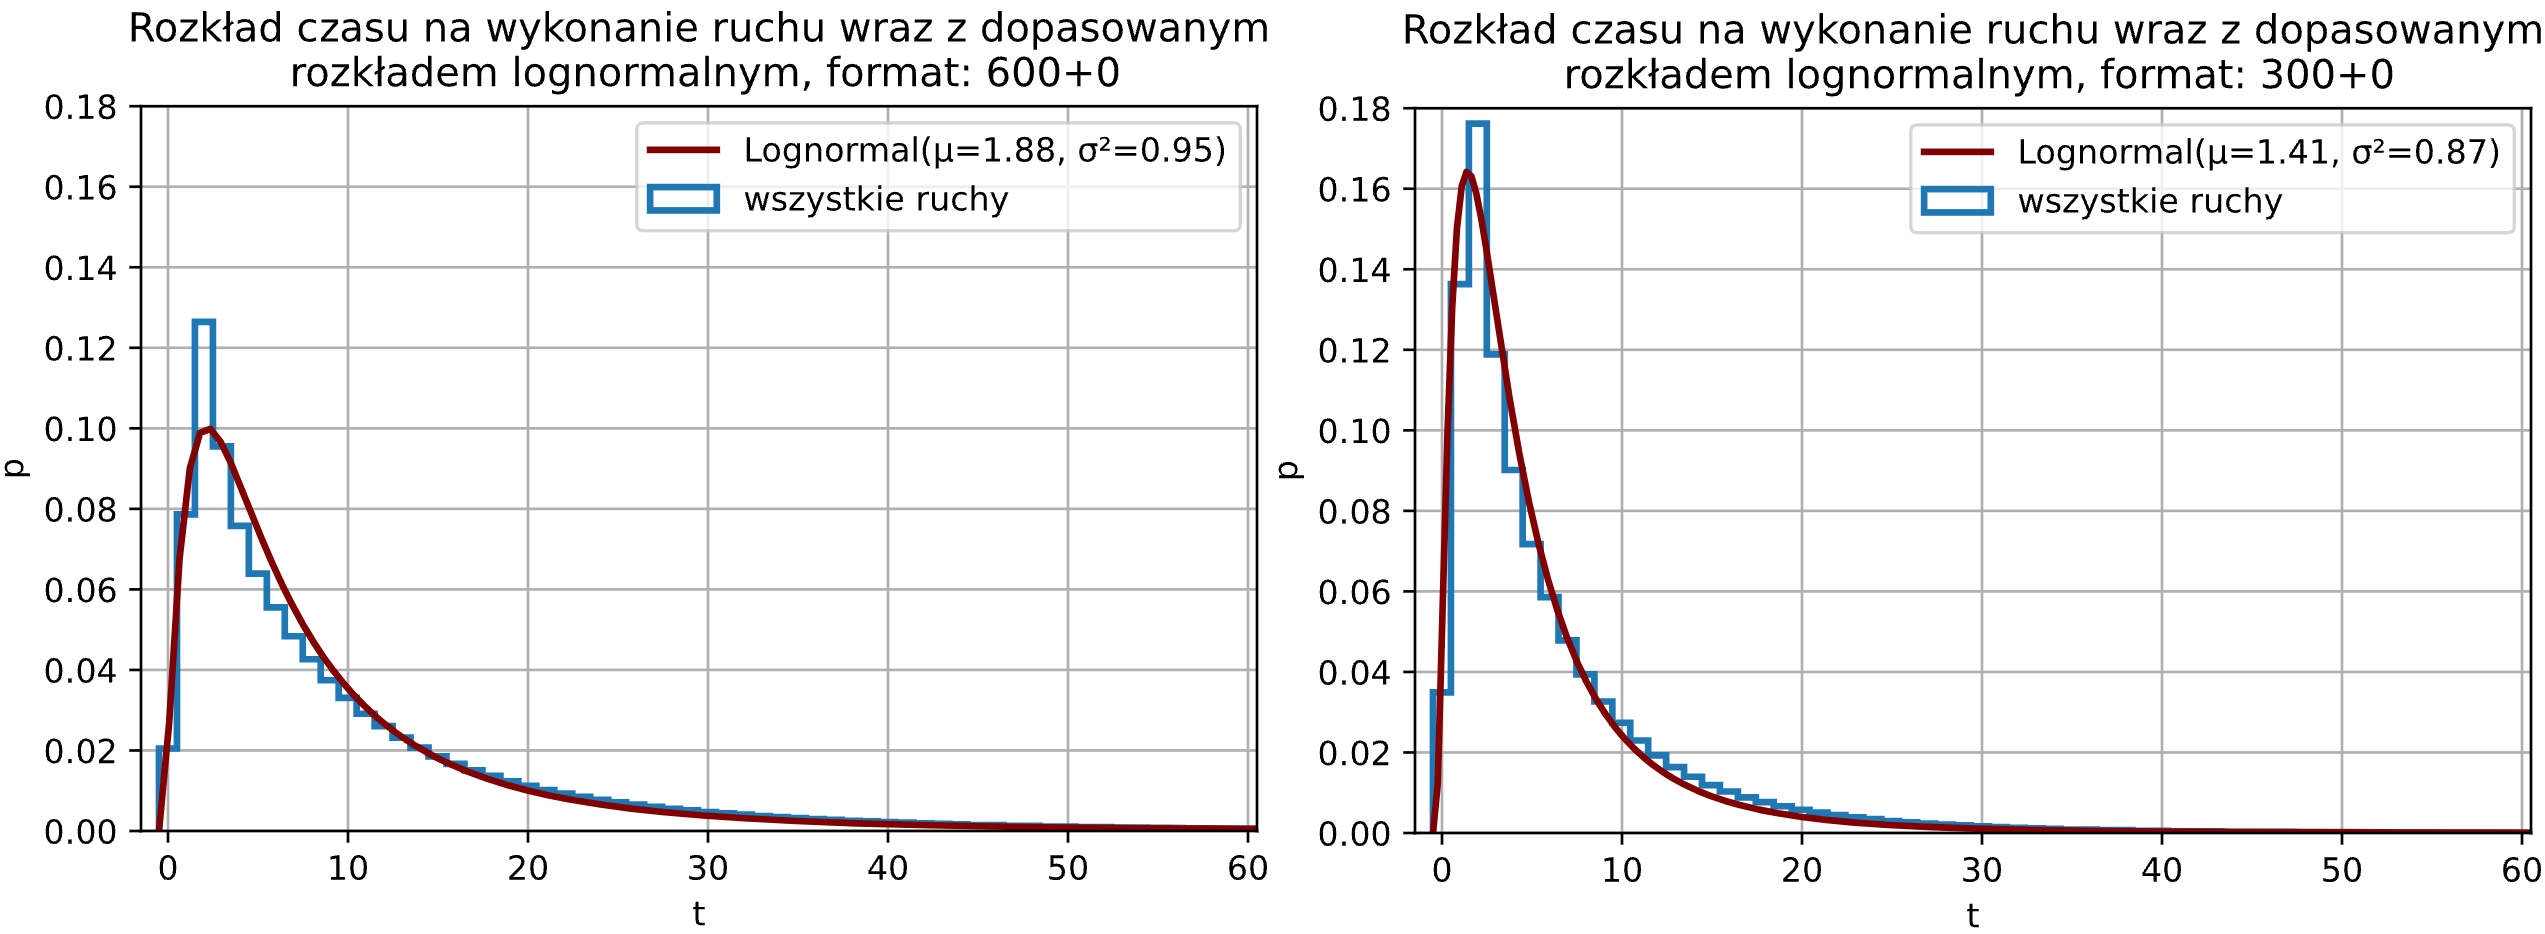
\includegraphics[width=\textwidth]{rozklad_lognorm.png}
	\caption{Rozkład czasu poświęconego na wykonanie posunięcia dla formatów ,,600+0'' i ,,300+0'' z dopasowanym rozkładem log-normalnym.}
	\label{rys:rozklad_lognorm}
\end{figure}
\begin{figure}[h]
	\centering
	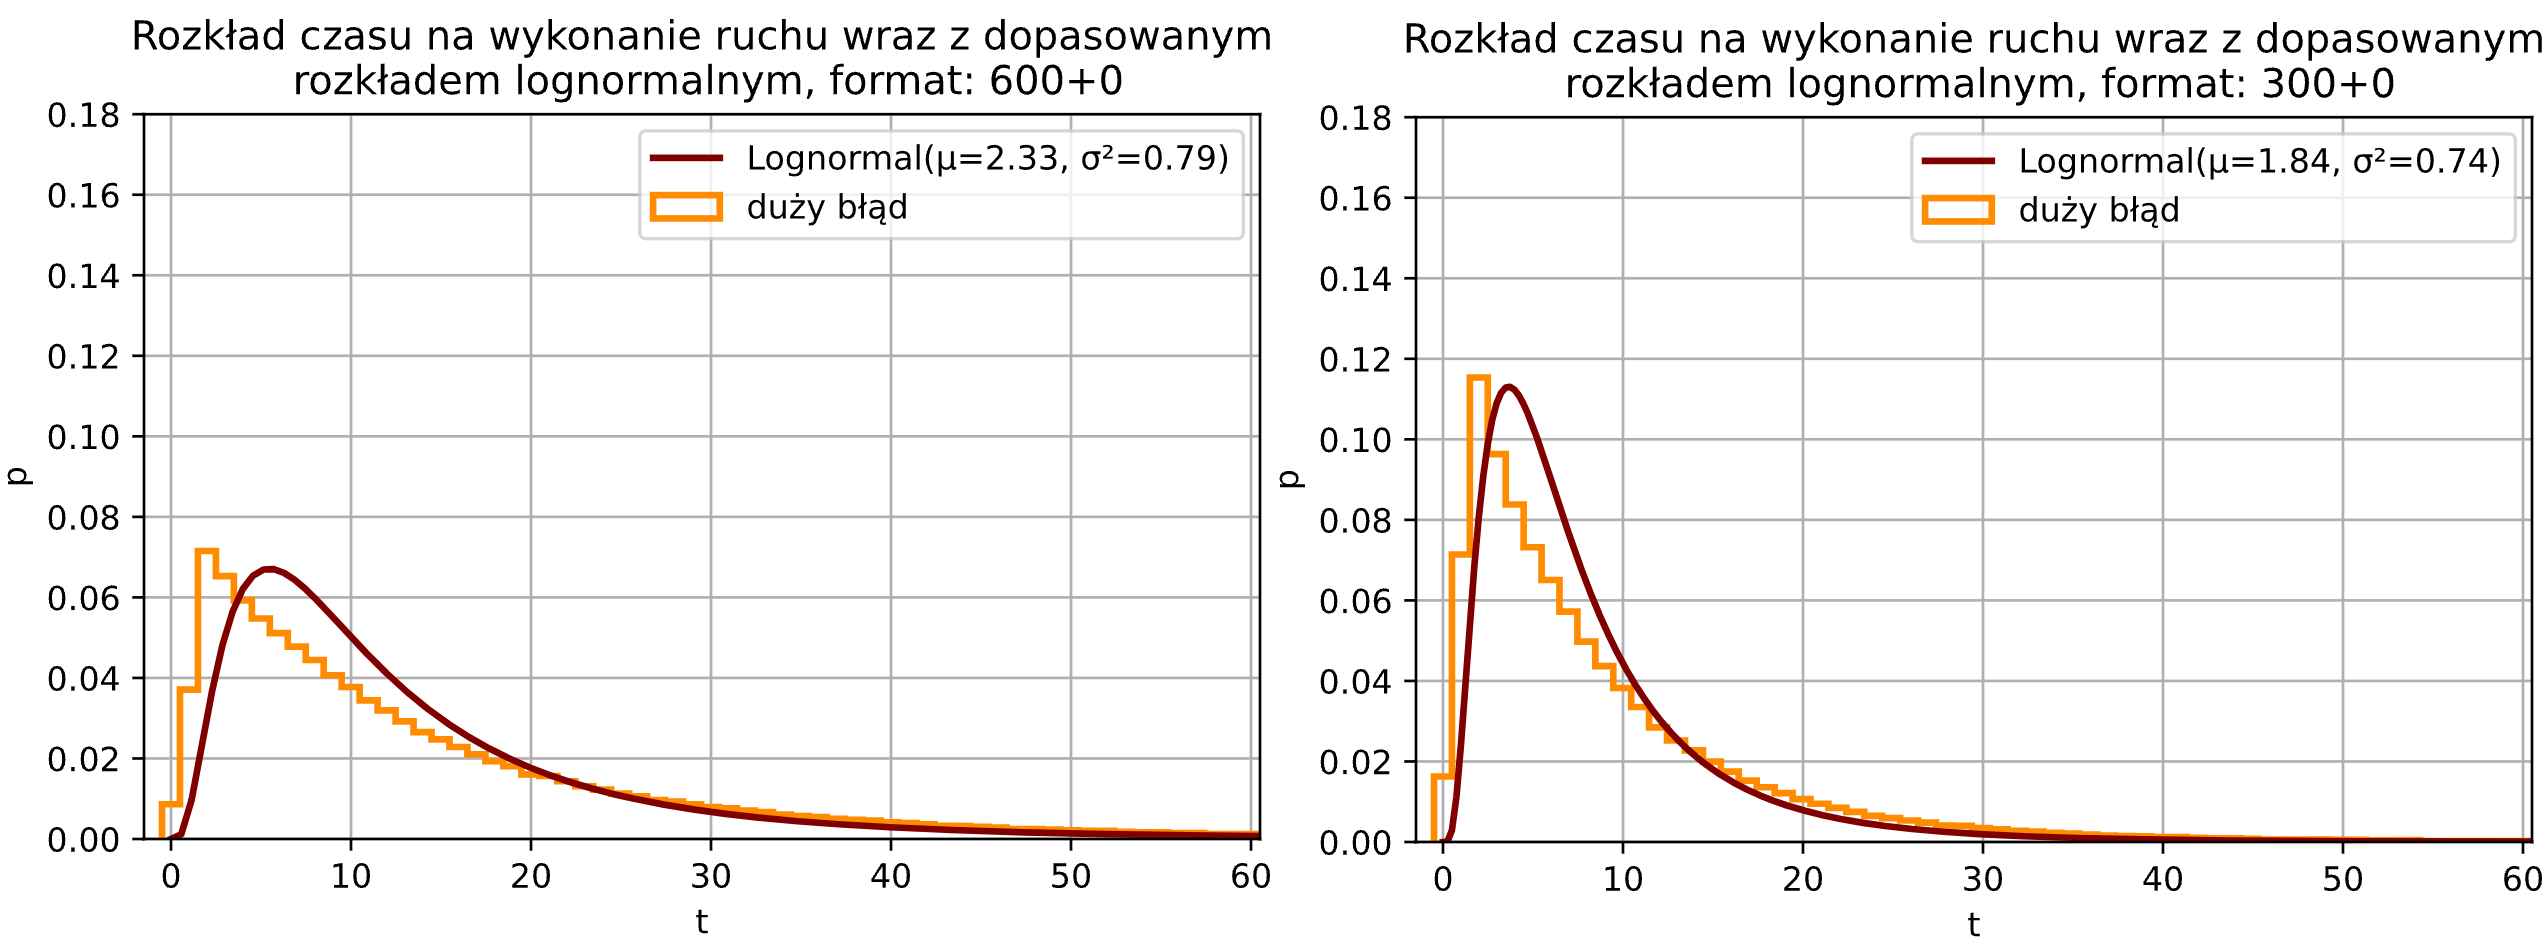
\includegraphics[width=\textwidth]{rozklad_lognorm2.png}
	\caption{Rozkład czasu poświęconego na wykonanie posunięcia dla formatów ,,600+0'' i ,,300+0'' z dopasowanym rozkładem log-normalnym. Zestaw ruchów błędnych.}
	\label{rys:rozklad_lognorm2}
\end{figure}
Za pomocą metody momentów opisanej w rozdziale na stronie \ref{teoria} do każdego zbioru danych został dopasowany rozkład log-normalny. Na rysunku \ref{rys:rozklad_lognorm} przedstawiającym znormalizowany histogram dla zestawu wszystkich ruchów dla formatów ,,300+0'' i ,,600+0'' rozkład teoretyczny jest dobrze dopasowany i zgodny z rozkładem empirycznym. Dla zestawu ruchów oznaczonych jako błędne, dopasowanie (rysunek \ref{rys:rozklad_lognorm2}) w dużym stopniu odbiega od rozkładu empirycznego. Ruchy błędne zajmują statystycznie mniej czasu, niż wskazuje rozkład. Ze względu na wielkość prób wynoszących od ponad 500 tysięcy obserwacji dla najmniejszego z analizowanych zbiorów (format ,,300+0'', ruchy błędne) do aż 8,6 miliona (format ,,600+0'', wszystkie ruchy), najpopularniejsze testy statystyczne, wrażliwe na liczbę danych odrzuciły hipotezę ich pochodzenia z rozkładu log-normalnego. Problematyczną kwestią jest tutaj również digitalizacja danych, które są zaokrąglane do pełnych sekund. W związku z powyższym zastosowane zostało kilka poprawek, by móc lepiej ustalić tożsamość danych.
Pierwszą z nich jest zmiana rozkładu log-normalnego na dyskretny rozkład lognormalny \cite{lognorm_disc}. Jest to drugi z opisanych rozkładów w tegorocznej pracy ,,Discrete lognormal distribution with application to insurence data'', którą napisali Jiahang Lyu oraz Saraless Nadarajah. Funkcja prawdopodobieństwa przedstawionego rozkładu opisana jest następującym wzorem
\begin{equation}\label{discrete}
	p_{X}(i)= \Phi\left(\frac{\log i - \mu}{\sigma} \right) - \Phi\left(\frac{\log \left(i - 1\right) - \mu}{\sigma} \right)
\end{equation}
gdzie $\Phi(x)$ jest wartością dystrybuanty standardowego rozkładu normalnego w punkcie $x$.
W celu estymacji parametrów $\mu$ i $\sigma$, z każdego ze wzorów wzięta została losowa próbka $(x_1, \dots, x_n)$ 100 tysięcy obserwacji, a następnie numerycznie znaleziona optymalna wartość funkcji największej wiarygodności opisanej równaniem
\begin{equation}
	L(\mu,\sigma) = \sum_{i=1}^{n} \log\left[ \Phi\left(\frac{\log x_i - \mu}{\sigma} \right) - \Phi\left(\frac{\log \left(x_i - 1\right) - \mu}{\sigma} \right)\right]
\end{equation}
W równaniu \ref{discrete} można zauważyć, że najniższą obserwacją należącą do dziedziny jest $i = 1$ sekunda. W związku z tym, przed estymacją parametrów rozkładu, z danych usunięte zostały ruchy, których zaokrąglony czas wykonania wynosi 0 sekund. Dodatkowo wartość $\log(0)$ traktowana jest jako $\lim\limits_{x \rightarrow 0^{+}}\log(x) = -\infty$. W związku z tym
\begin{equation*}
	p_{X}(1) = \Phi\left(\frac{\log 1 - \mu}{\sigma} \right) - \Phi\left(\frac{\log \left(0\right) - \mu}{\sigma} \right) = \Phi\left(\frac{- \mu}{\sigma} \right).
\end{equation*}
 Wyniki obserwacji przedstawione są na rysunkach \ref{rys:lognorm_disc} oraz \ref{rys:lognorm2_disc}. Na pierwszym z nich, zawierającym zestaw wszystkich ruchów, dyskretny rozkład normalny jest dobrze dopasowany w obydwu formatach czasowych. Także w przypadku zestawu ruchów błędnych (rys. \ref{rys:lognorm2_disc}) dopasowanie poprawiło się w znacznym stopniu względem rozkładu ciągłego. Wykonany został test Chi-kwadrat badający zgodność częstotliwości występujących w danych z tymi zadanymi przez rozkład. Dla losowych zestawów danych liczących 1000 próbek i po wykonaniu 100 prób Monte-Carlo, średnia p-wartość dla każdego z badanych zbiorów na poziomie istotności $\alpha = 0,05$ wskazuje na przyjęcie hipotezy zerowej mówiącej o pochodzeniu danych z dyskretnego rozkładu log-normalnego. Szczegółowe wyniki, wraz z wyznaczonymi wcześniej za pomocą metody największej wiarygodności parametrami rozkładu umieszczone są w tabeli \ref{tab:testy}. Na podstawie średniej p-wartości da się zauważyć, że pomimo zgodności dopasowania do każdego ze zbiorów, zestaw wszystkich ruchów jest lepiej opisany przez zadany rozkład teoretyczny, niż zestaw ruchów błędnych. Potwierdzają to odchylenia w okolicy ruchów z indeksem od 3 do 8 na rysunku \ref{rys:lognorm2_disc}, które są zauważalnie większe, niż odchylenia w zbiorze wszystkich ruchów na rysunku \ref{rys:lognorm_disc}.

\begin{figure}[h]
	\centering
	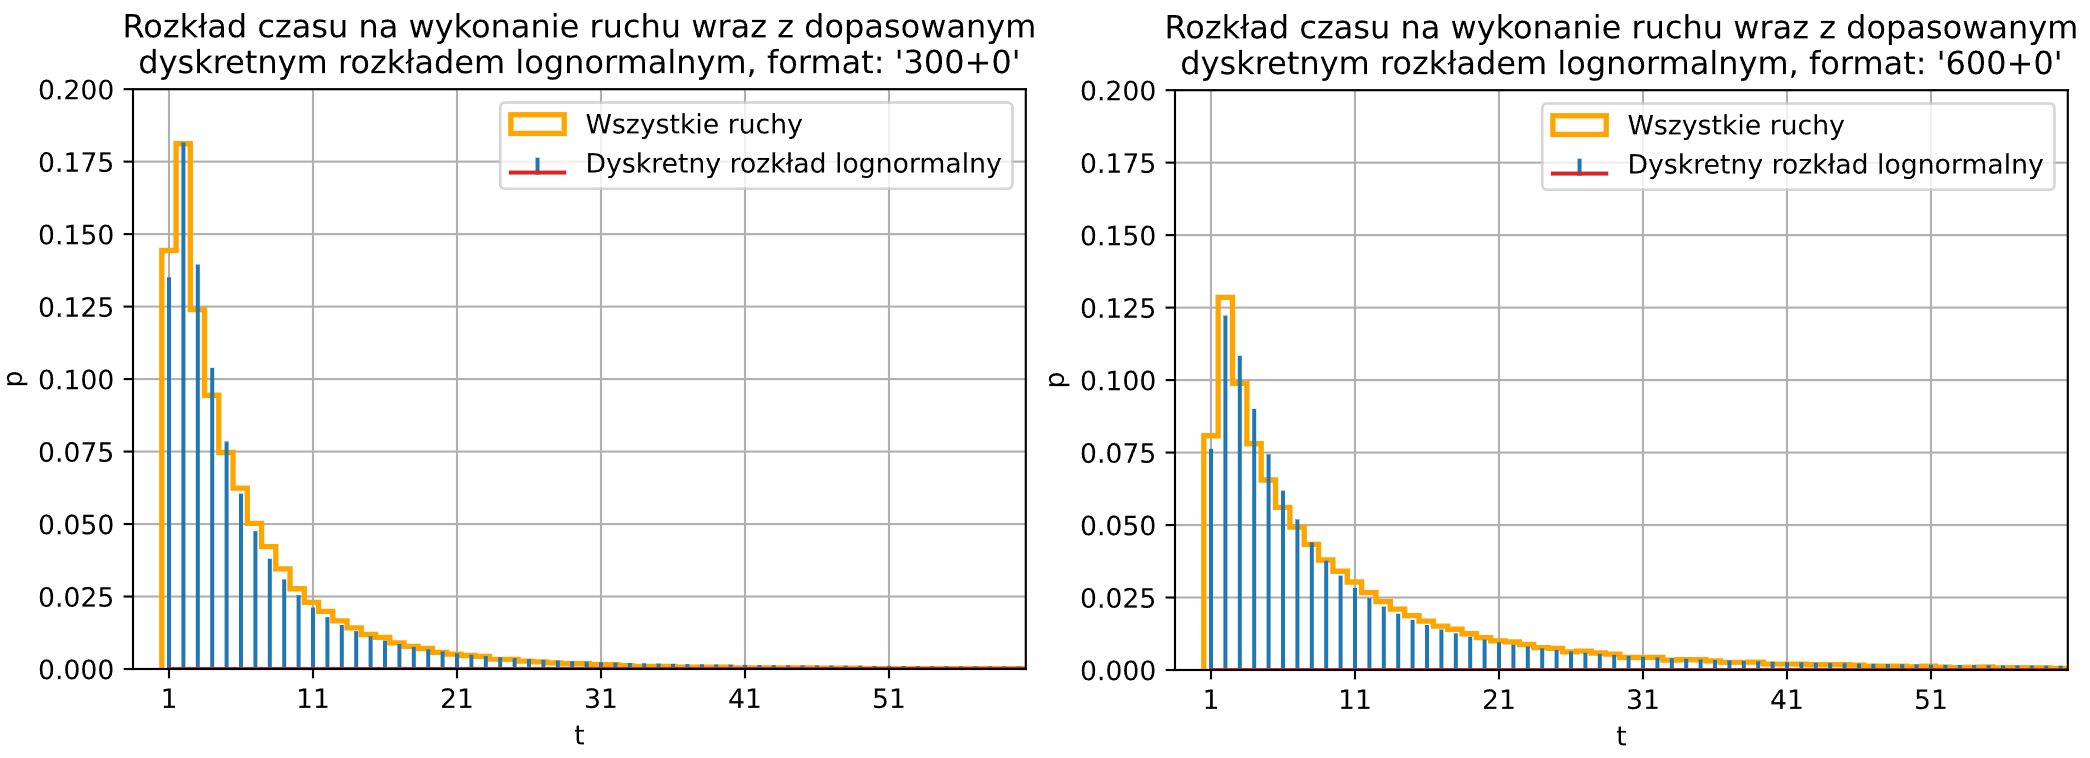
\includegraphics[width=\textwidth]{discrete_lognorm_1.png}
	\caption{Rozkład czasu poświęconego na wykonanie posunięcia dla formatów ,,600+0'' i ,,300+0'' z dopasowanym dyskretnym rozkładem log-normalnym.}
	\label{rys:lognorm_disc}
\end{figure}
\begin{figure}[h]
	\centering
	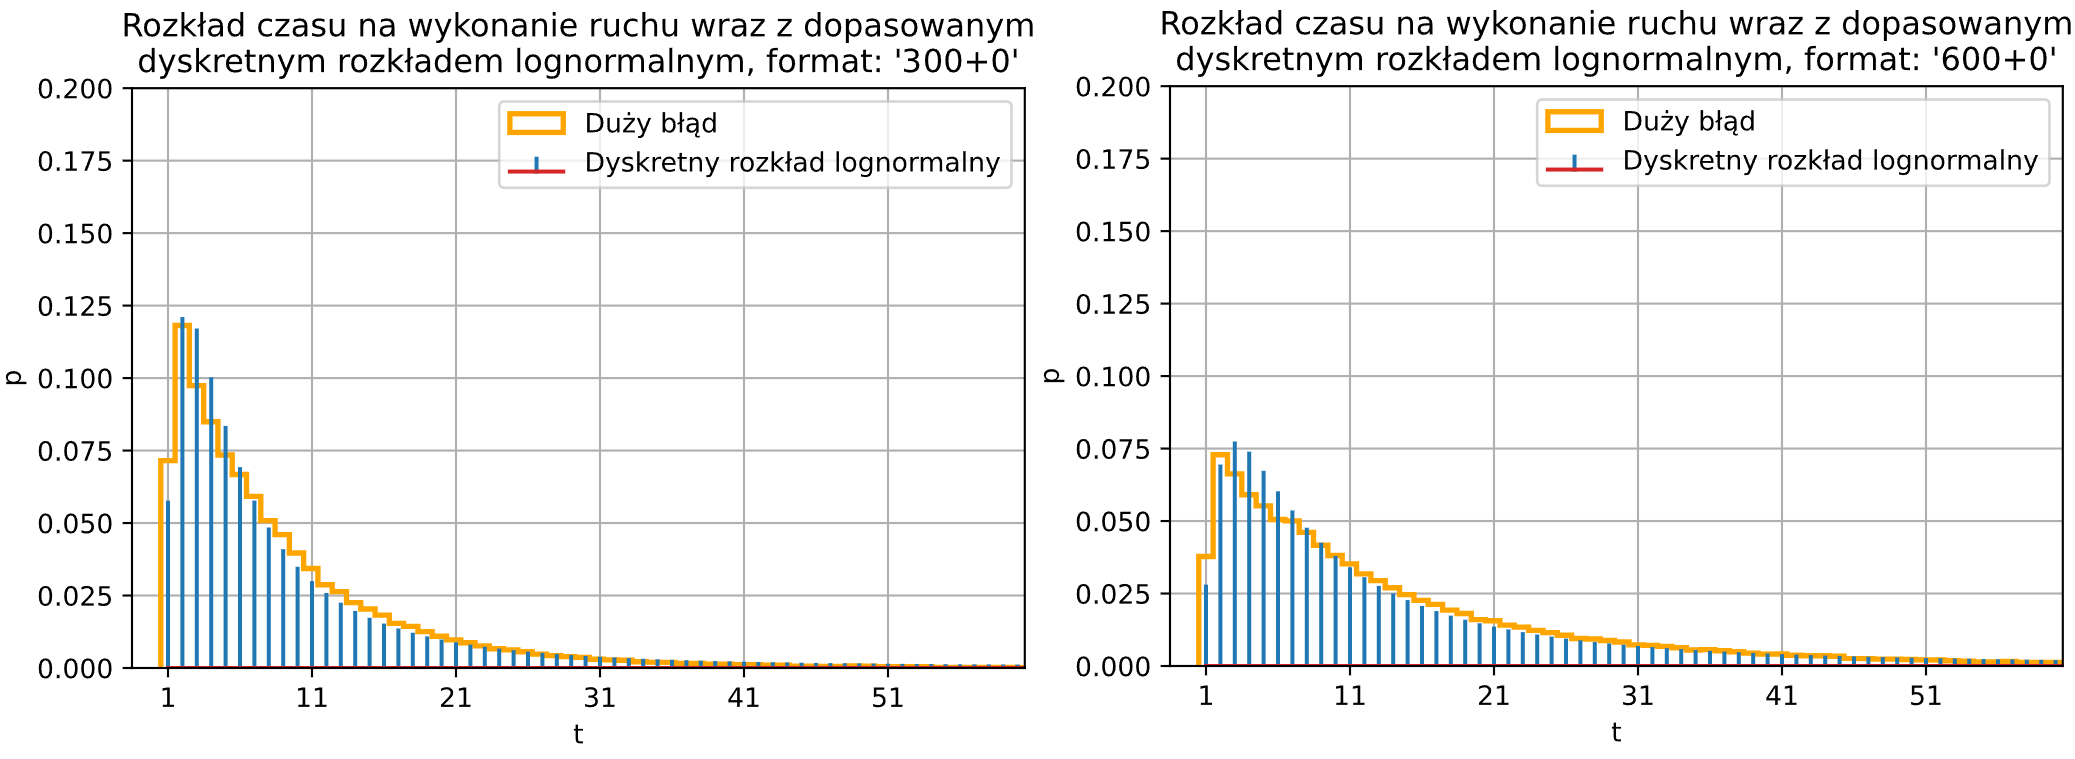
\includegraphics[width=\textwidth]{discrete_lognorm_2.png}
	\caption{Rozkład czasu poświęconego na wykonanie posunięcia dla formatów ,,600+0'' i ,,300+0'' z dopasowanym dyskretnym rozkładem log-normalnym. Zestaw ruchów błędnych.}
	\label{rys:lognorm2_disc}
\end{figure}

\begin{table}[h]
	\caption{Średnie wyniki testu zgodności Chi-kwadrat, średnia ze 100 prób Monte-Carlo dla losowych próbek o długości 1000. Poziom istotności $\alpha = 0,05$.}
	\centering
	\begin{tabular}{|l|l|l|l|}
		\hline
		\textbf{dane}                     & \textbf{parametry rozkładu}& \textbf{p-wartość} & \textbf{wynik}     \\ \hline
		,,300+0'', wszystkie ruchy & $\mu = 1,220$, $\sigma = 1,091$& 22,28\%                    & przyjęcie hipotezy \\ \hline
		,,600+0'', wszystkie ruchy & $\mu = 1,705$, $\sigma = 1,188$& 20,40\%                    & przyjęcie hipotezy \\ \hline
		,,300+0'', ruchy błędne    & $\mu = 1,673$, $\sigma = 1,059$& 7,14\%                     & przyjęcie hipotezy \\ \hline
		,,600+0'', ruchy błędne    & $\mu = 2,158$, $\sigma = 1,123$& 6,49\%                     & przyjęcie hipotezy \\ \hline
	\end{tabular}
	\label{tab:testy} 
\end{table}

\chapter{Podsumowanie}
Na podstawie bazy danych ze strony \textit{Lichess.com} dotyczących 17 524 012 posunięć ze 275 994 gier rozgrywanych na każdym poziomie rankingowym w formatach ,,300+0'' oraz ,,600+0'' zbadane zostało kilka statystyk i zależności związanych z szachami szybkimi. Pokrótce opisane zostaną teraz najważniejsze analizy, a także wnioski z nich płynące.

Po wstępnym przygotowaniu danych i wyznaczeniu pierwszych statystyk, w pracy został określony został empiryczny rozkład długości gry. Niecałe 5\% gier z rozpatrywanych formatów czasowych zawiera więcej niż 57 ruchów. 

Przy badaniu zależności pomiędzy indeksem ruchu, a czasem poświęconym na posunięcie określony został średni czas na wykonanie posunięcia w zależności od jego indeksu. W obydwu formatach dla każdego numeru ruchu błędne posunięcia zajmowały średnio więcej czasu porównując z zestawem wszystkich ruchów, a także miały większą wariancję.
Zaproponowana została przyczyna takiego stanu, mianowicie zarówno szansa na popełnienie błędu jak i czas na wykonanie posunięcia mogą być silnie zależne od stopnia skomplikowania pozycji, a wśród zestawu wszystkich ruchów średnia może być zaniżana przez ruchy oczywiste i forsowne (tylko jeden możliwy legalny ruch), które zajmują statystycznie mniej czasu.
Analiza zależności pomiędzy numerem ruchu, a średnim poświęconym czasem została również przeprowadzona z podziałem na poszczególne grupy rankingowe. Dla każdego analizowanego formatu czasowego gracze z wyższym rankingiem mają tendencję do szybszego wykonywania początkowych posunięć, będących zazwyczaj elementem teorii otwarć szachowych, dla których szansa na popełnienie błędu jest najmniejsza. Zauważalnie dłużej natomiast wykonują posunięcia z indeksem od 20 do 30 - czyli te, gdzie prawdopodobieństwo popełnienia błędu jest największe, a nieznacznie dłużej ruchy z indeksem od 30. Dla zestawu ruchów błędnych, wyżej notowani gracze poświęcają na posunięcie zdecydowanie więcej czasu. Czas wydzielony na ruchy z największym prawdopodobieństwem na popełnienie błędu sprawia, że różnica w częstotliwości popełniania błędów pomiędzy lepszymi, a gorszymi graczami dla gry środkowej jest bardzo duża. Przy posunięciach z indeksem powyżej 40, szansa na pomyłkę jest podobna dla każdego rankingu. 25\% Najsłabszych graczy ma tendencję do popełniania nawet kilkukrotnie większej liczby błędów w ruchach z indeksem poniżej 10, niż ich wyżej notowani rywale. Wysuwa to wniosek, że nauka otwarć szachowych (wiążąca się z mniejszą liczbą błędów w początkowej fazie gry) może pozwolić początkującym zawodnikom na skuteczniejsze zdobycie punktów rankingowych.

Badanie zależności pomiędzy formatem ,,300+0'' i ,,600+0'' pokazało kilka ciekawych cech. w formacie ,,600+0'' gracze mają do dyspozycji dokładnie dwa razy więcej czasu, niż w dla ,,300+0'', jednakże czas poświęcony na konkretny ruch nie jest prawie nigdy dwukrotnie większy. Dla zbioru wszystkich ruchów w początkowej fazie gry posunięcia w dłuższym formacie trwają średnio około 1,65 raza dłużej z tendencją rosnącą liniowo wraz ze wzrostem indeksu, aż do okolic 1,8 raza dłużej przy ruchach z indeksem powyżej 50. Natomiast stosunek czasu dla ruchów oznaczonych przez silnik jako błędne zachowuje podobne wartości do zestawu wszystkich ruchów w początkowej fazie gry, w przypadku gry końcowej jest jednak znacznie większy i dochodzi 2. Wiąże się to z większą średnią pozostałą procentową ilością czasu w formacie ,,600+0'', dzięki której zawodnik może pozwolić sobie na dłuższe zastanowienie się w późniejszej fazie meczu.

Prawdopodobieństwo popełnienia błędu w konkretnym ruchu jest bardzo zbliżone w obydwu analizowanych formatach w początkowej fazie gry. Od ruchu 20, szansa na błąd jest nieznacznie większa w krótszym formacie. Różnica prawdopodobieństwa na wykonanie choć jednego błędu w pierwszych 10, 20 lub 30 ruchach, przy założeniu niezależności ruchów jest mała. Mimo większej ilości czasu w formacie ,,600+0'', błędów w początkowej fazie gry pojawia się statystycznie nieznacznie więcej niż w krótszym formacie. Znacząca różnica jest natomiast widoczna pomiędzy poszczególnymi przedziałami rankingowymi. 25\% najgorzej radzących sobie graczy ma ponad 40\% szansy na błąd w pierwszych 10 ruchach, natomiast w przypadku graczy z rankingiem plasującym się pomiędzy 25, a 50 centylem jest to o prawie połowę mniej.

Ostatnią analizowaną zależnością jest rozkład czasu poświęconego na wykonanie posunięcia, osobno dla zbioru wszystkich ruchów i dla oznaczonych przez silnik jako błędne. Dla obu formatów najwięcej posunięć zajmuje od jednej do pięciu sekund, by stopniowo maleć dla większej ilości czasu. Dominanta dla wszystkich zestawów wynosi 2, jednakże dla ruchów błędnych, histogram częstotliwości wystąpienia jest bardziej spłaszczony. Rozkład danych dla każdego zestawu jest wizualnie dobrze opisany przez rozkład log-normalny, a jeszcze lepiej - w związku z tym, że dane są dyskretne, przez dyskretny rozkład lognormalny z parametrami estymowanymi metodą największej wiarygodności. Potwierdza to test zgodności Chi-kwadrat.

Powyższe analizy i rozważania mogą zostać uzupełnione w dalszej pracy o inne formaty czasowe, ze szczególnym uwzględnieniem tych z czasem dodawanym po posunięciu. Dodatkowo, można wprowadzić miarę skomplikowania pozycji i uwzględnienia jej wpływu na wyniki analiz, wymaga to jednak dużej mocy obliczeniowej i dokładnego zbadania poszczególnych posunięć w każdej z analizowanych partii.

%\begin{itemize}
%	\item 95\% gier kończy się w 57 ruchach 
%	\item błąd dla każdego elo dla każdego posunięcia zajmuje średnio dłużej, ma też zawsze większą wariancje 
%	\item wszystkie ruchy: lepsi gracze szybciej wykonują ruchy początkowe, dłużej te z największą szansą na błąd (ok 20) 
%	\item największa szansa na błąd -- okolice 20 ruchu 
%	\item odnośnie dwóch poprzednich, lepsi gracze najmniej popełniają błędów w okolicach 20 ruchu 
%	\item największa szansa na błąd -- różnice dla elo (dużo błędów na początku 
%	dla słabych graczy pozniej sie stabilizuje) 
%	\item lepsi gracze DŁUŻEJ wykonują ruchy BŁĘDNE
%	\item różnice między formatami - w 600+0 ruchy zajmują nieliniowo więcej czasu, w 300+0 gracze są zmuszeni szybko wykonywać ruchy późniejsze.
%	\item 10 pierwszych ruchów, istotna różnica w popełnieniu rażącego błędu między graczami słabymi a dobrymi
%\end{itemize}


%%%%%%%%%%%%%%%%%%%%%%%%%%%%%%%%%%%%%%%%%%%%%%%%%%%%%%%%%
% BIBLIOGRAFIA
% W tworzeniu bibliografii najlepiej korzystać z BibTex'a, 
% który jest częścią systemu Tex. W naszym przypadku funkcję 
% przechowalni literatury, do której się odwołujemy, pełni 
% plik bibliografia.bib. Nie musimy ręcznie dodawać nowych 
% pozycji do bibliografii. Możemy wejść np. na stronę 
% https://mathscinet.ams.org/mathscinet/index.html, 
% znaleźć odpowiednią pozycję, wybrać ją, a następnie zmienić 
% 'Select alternative format' na BibTeX, skopiować uzyskany 
% tekst, wkleić do pliku bibliografia.bib i skompilować. 
% Gotowe informacje do pliku bibliografia.bib można znaleźć 
% także na https://arxiv.org - gdy znajdziemy interesującą nas 
% pracę, szukamy 'References & Citations' i klikamy 'NASA ADS', 
% a potem 'Bibtex entry for this abstract' 
% i postępujemy tak jak wcześniej.
%%%%%%%%%%%%%%%%%%%%%%%%%%%%%%%%%%%%%%%%%%%%%%%%%%%%%%%%%
\newpage
% w nawiasie klamrowym wpisujemy nazwę pliku z bibliografią w formacie .bib
\bibliography{bibliografia} 
\end{document}